\documentclass[twoside,a4paper,12pt]{extreport} %,draft,openright

\usepackage[utf8]{inputenc}
\usepackage[T1]{fontenc}
\usepackage[MeX]{polski}
\usepackage{gensymb}
\usepackage{epsf}

\newif\ifpdf
\ifx\pdfoutput\undefined
\pdffalse
\else
\pdfoutput=1
\pdftrue
\fi
\ifpdf
\usepackage[pdftex]{graphicx}
\pdfcompresslevel=9
\else
\usepackage{graphicx}
\fi
\usepackage{mdwlist}
\usepackage{subfigure}
\usepackage{latexsym,amssymb}
\usepackage{setspace,cite}
\usepackage{indentfirst}
\usepackage{mathtools}
\usepackage{url}
%% #### Ustawianie łamania linii dla adresów URL podawanych w bibliografii #### %%
\usepackage{breakurl}
\usepackage[breaklinks]{hyperref}
\def\UrlBreaks{\do\/\do-}
%% #################################################################### %%
\usepackage[justification=centering]{caption}
\newcommand{\source}[1]{\vspace{-0.3cm}\caption*{\small Źródło: \url{#1}} }
\usepackage{multirow}
\usepackage[figuresright]{rotating}
\usepackage{csquotes}
\usepackage{listings,xcolor}
\usepackage{float}
\usepackage[T1]{fontenc}
\usepackage{mathptmx}
\usepackage{layout}
\usepackage{verbatim}
\newfloat{lstfloat}{htbp}{lop}
\floatname{lstfloat}{Listing}
\usepackage{enumitem}
\usepackage{minted}

%% ############### JSON listing's style definition ############### %%
\colorlet{punct}{red!60!black}
\definecolor{background}{HTML}{EEEEEE}
\definecolor{delim}{RGB}{20,105,176}
\colorlet{numb}{magenta!60!black}

\lstdefinelanguage{json}{
    basicstyle=\fontsize{9}{9}\ttfamily,
    showstringspaces=false,
    breaklines=true,
    string=[s]{"}{"},
    stringstyle=\color{orange},
    literate=
     *{0}{{{\color{numb}0}}}{1}
      {1}{{{\color{numb}1}}}{1}
      {2}{{{\color{numb}2}}}{1}
      {3}{{{\color{numb}3}}}{1}
      {4}{{{\color{numb}4}}}{1}
      {5}{{{\color{numb}5}}}{1}
      {6}{{{\color{numb}6}}}{1}
      {7}{{{\color{numb}7}}}{1}
      {8}{{{\color{numb}8}}}{1}
      {9}{{{\color{numb}9}}}{1}
      {:}{{{\color{punct}{:}}}}{1}
      {,}{{{\color{punct}{,}}}}{1}
      {\{}{{{\color{delim}{\{}}}}{1}
      {\}}{{{\color{delim}{\}}}}}{1}
      {[}{{{\color{delim}{[}}}}{1}
      {]}{{{\color{delim}{]}}}}{1},
}
%% #################################################################### %%
\def\lstfloatautorefname{Listing} % needed for hyperref/auroref

\newenvironment{bottompar}{\par\vspace*{\fill}}{\clearpage}
\BeforeBeginEnvironment{figure}{\vskip-2ex}
\AfterEndEnvironment{figure}{\vskip-1ex}
\lstset{showstringspaces=false}

% for margins left, right top bottom
\usepackage{anysize}
\marginsize{3cm}{2.5cm}{2.5cm}{2.5cm}
\let\origdoublepage\cleardoublepage    %%komenda wstawiająca czyste kartki
\newcommand{\clearemptydoublepage}{%
  \clearpage
  {\pagestyle{empty}\origdoublepage}%
}
\let\cleardoublepage\clearemptydoublepage


%\usepackage{draft} %draft option - doesn't put full figures in -
            % useful when editing
%does the headers on the pages - keep in
\usepackage{fancyhdr}

%omitting any of these makes the thesis compile without the omitted
%chapter - good for editing single chapters.
%\includeonly{header,appendix}

\usepackage{etoolbox}% http://ctan.org/pkg/etoolbox
\makeatletter
\patchcmd{\@makechapterhead}{\vspace*{50\p@}}{}{}{}% Removes space above \chapter head
\makeatother
\usepackage{titlesec}
\titlespacing\section{0pt}{4pt plus 1pt minus 2pt}{0pt plus 1pt minus 2pt}
\titlespacing\subsection{0pt}{4pt plus 0.5pt minus 2pt}{0pt plus 0.5pt minus 2pt}
\titlespacing\subsubsection{0pt}{4pt plus 0.5pt minus 2pt}{0pt plus 0pt minus 2pt}
\begin{document}
\DeclareGraphicsExtensions{.pdf,.png,.eps}
\newpage

%Puts page numbering of preamble in roman and of main body of thesis in
%arabic. Also defines how chapters and sections are made
\pagenumbering{arabic}
\setcounter{page}{1} \pagestyle{fancy}
\renewcommand{\chaptermark}[1]{\markboth{\chaptername%
\ \thechapter:\,\ #1}{}}
\renewcommand{\sectionmark}[1]{\markright{\thesection\,\ #1}}

%DEFINES TITLE PAGE, and contains abstract, acknowledgements, etc.

\newpage
\thispagestyle{empty}

% ******* Title page *******
% **************************
\begin{onehalfspacing}
\begin{center}

\centering
\title{Praca magisterska}
\author{Autor: Grzegorz Galios}

{\fontsize{17}{17}}\selectfont
\textsc{Uniwersytet Śląski w Katowicach \\[.3cm]
Wydział Nauk Ścisłych i Technicznych  \\[.3cm]
Informatyka  \\[2.5cm]}
\textbf{\large{Grzegorz Galios}} \\
315850\\[1cm]

\large 
{Zastosowanie konwolucyjnej sieci neuronowej w procesie sterowania samochodem w symulowanym środowisku} \\[.5cm]
\textsc{Praca dyplomowa magisterska}
\end{center} ~\\[3cm]

\large
\begin{flushright}
Promotor: dr Rafał Skinderowicz \\
\end{flushright}

\begin{bottompar}
\begin{flushright}
Katowice, 2022
\end{flushright}
\end{bottompar}
\end{onehalfspacing}

\pagenumbering{Roman}
\setcounter{page}{0} \pagestyle{plain}

\pagestyle{fancy}


\newpage
Słowa kluczowe: \hspace{0.5cm} \textit{konwolucyjne sieci neuronowe, uczenie ze wzmocnieniem} \\[1cm]
\textbf{Oświadczenie autora pracy}\\

Ja, niżej podpisany: \\

\hspace{1.5cm} imię (imiona) i nazwisko: Grzegorz Galios \\

\hspace{1.5cm} autor pracy dyplomowej pt. 
\textit{„Zastosowanie konwolucyjnej sieci neuronowej w procesie sterowania samochodem w symulowanym środowisku”}\\

Numer albumu: 315850 \\

Student Wydziału Nauk Ścisłych i Technicznych Uniwersytetu Śląskiego w Katowicach \\ 

kierunku studiów: Informatyka - niestacjonarne II stopnia \\

specjalności: Inteligentne Systemy Informatyczne \\

Oświadczam, że w/w. praca dyplomowa:   
\begin{itemize}
\item została przygotowana przeze mnie samodzielnie$^1$,  
\item nie narusza praw autorskich w rozumieniu ustawy z dnia 4 lutego 1994 r. o prawie autorskim i prawach pokrewnych (tekst jednolity Dz. U. z 2006 r. Nr 90, poz. 631, z późn. zm.) oraz dóbr osobistych chronionych prawem cywilnym,  
\item nie zawiera danych i informacji, które uzyskałem w sposób niedozwolony,  
\item nie była podstawą nadania dyplomu uczelni wyższej lub tytułu zawodowego ani mnie, ani innej osobie.  
\end{itemize}
Oświadczam również, że treść pracy dyplomowej zamieszczonej przeze mnie w Archiwum Prac Dyplomowych jest identyczna z treścią zawartą w wydrukowanej wersji pracy. \\[0.5cm]
\textbf{Jestem świadomy odpowiedzialności karnej za złożenie fałszywego oświadczenia.} \\[1.5cm]

\begin{minipage}{0.4\textwidth}
\begin{flushleft}
\centering
\textbf{...............................}\\
\textbf{Data}
\end{flushleft}
\end{minipage}
\begin{minipage}{0.4\textwidth}
\begin{flushright}
\textbf{...............................}\\
\textbf{Podpis autora pracy}
\end{flushright}
\end{minipage} \\[1cm]
$^1$ uwzględniając merytoryczny wkład promotora (w ramach prowadzonego seminarium dyplomowego)

\addtocontents{toc}{\protect\setcounter{tocdepth}{1}}
\setcounter{secnumdepth}{2}
\tableofcontents
\newpage

%sets up headers for lefthand and righthand pages.
\pagenumbering{arabic}
\fancyhead[LE,RO]{\slshape \rightmark}
\fancyhead[LO,RE]{\slshape \leftmark}
\fancyfoot[C]{\thepage}

\setlength{\parskip}{1ex} %odstępy między akapitami
\onehalfspacing

\chapter*{Wstęp}
\addcontentsline{toc}{chapter}{Wstęp}
Przedmiotem pracy jest zastosowanie konwolucyjnej sieci neuronowej oraz technik głębokiego uczenia maszynowego do rozwiązania problemu sterowania samochodem autonomicznym. Ponieważ jest to bardzo złożone zagadnienie, dlatego wiele uwagi zostało poświęconej na potrzeby dobrego zrozumienia jego podstawowych elementów.

\vspace*{1.5cm}
\section*{Cel i zakres pracy}
Jako cel pracy przyjęto opracowanie prostego systemu uczącego konwolucyjne sieci neuronowe w oparciu o symulacje uruchamiane w przygotowanym środowisku wirtualnym. Sieć neuronowa rozwiązuje problem jazdy samochodem po torze wyścigowym w oparciu o obraz z kamer zamontowanych w samochodzie. \\
Zakres pracy obejmuje poniższe zagadnienia:
\begin{enumerate*}
\item Przegląd literatury na temat samochodów autonomicznych, wykorzystywanych typów czujników oraz wiodących rozwiązań na rynku.
\item Przegląd literatury na temat konwolucyjnych sieci neuronowych.
\item Zaprojektowanie systemu uczącego konwolucyjne sieci neuronowe oraz wybór odpowiednich narzędzi do jego implementacji.
\item Implementacja systemu uczącego konwolucyjne sieci neuronowe w oparciu o obraz z kamer zamontowanych w wirtualnym samochodzie oraz inne sygnały płynące ze środowiska symulacji.
\item Przeprowadzenie eksperymentów obliczeniowych na utworzonym systemie oraz analiza uzyskanych wyników.
\end{enumerate*}

\newpage
\section*{Struktura pracy}
Praca jest złożona z pięciu numerowanych rozdziałów, a każdy z nich dotyczy określonego elementu omawianego tematu. Kolejność rozdziałów jest realizacją zasady ,,\textit{od ogółu do szczegółu}'' - praca rozpoczyna się od omówienia teoretycznych pojęć, niezbędnych do zrozumienia jej dalszej treści. Natomiast dwa ostatnie rozdziały dotyczą bardzo konkretnych oraz praktycznych zagadnień. Lista rozdziałów przedstawia się następująco:
\begin{enumerate*}
\item \textbf{Samochody autonomiczne} \\
Rozdział opisuje problematykę zagadnienia samochodów autonomicznych, kładąc szczególny nacisk na zaprezentowanie oraz porównanie ze sobą urządzeń wykorzystywanych w modelu percepcji samochodów. Pokaźna część rozdziału została poświęcona opisaniu wiodących rozwiązań oferowanych obecnie na rynku.
\item \textbf{Konwolucyjne sieci neuronowe} \\
Rozdział zawiera najistotniejsze zagadnienia teoretyczne z zakresu konwolucyjnych sieci neuronowych, ich treningu oraz obszaru zastosowań. Przedstawione zagadnienia to niezbędne minimum, potrzebne do prawidłowego zrozumienia dalszej części pracy.
\item \textbf{Projekt systemu i opis narzędzi} \\
Rozdział został podzielony na dwie części. W pierwszej z nich zostały opisane główne założenia projektowe dla implementowanego systemu. Z kolei w części drugiej zamieszczono opis narzędzi wykorzystanych podczas implementacji systemu.
\item \textbf{Opis implementacji} \\
Rozdział przedstawia opis implementacji systemu wykonanego na potrzeby tej pracy. Szczególny nacisk został położony na opisanie kluczowych komponentów wchodzących w skład systemu.
\item \textbf{Eksperymenty obliczeniowe} \\
Rozdział poświęcony na przedstawienie metodyki przeprowadzanych eksperymentów obliczeniowych oraz analizę uzyskanych wyników.
\end{enumerate*}
\chapter{Samochody autonomiczne}
\vspace{-1cm}
Samochody autonomiczne są pojazdami, które mają zdolność do interpretacji swojego otoczenia i bezpiecznego poruszania się po nim przy jak najmniejszej ingerencji człowieka siedzącego na fotelu kierowcy. Poziom automatyzacji sterowania może się różnić dla poszczególnych modeli. Organizacja SAE (\textit{Society of Automotive Engineers}) zdefiniowała sześć poziomów automatyzacji sterowania samochodem \cite{synopsys:whatIsAutonomousCar}. W pełni autonomiczne samochody mają być całkowicie pozbawione kierownicy, pedałów oraz innych przyrządów tradycyjnie używanych do sterowania ręcznego.

W chwili obecnej nie istnieje ani jeden model w pełni autonomicznego samochodu, dopuszczonego do produkcji seryjnej. Co więcej, niewiele wskazuje na to, żeby taki stan rzeczy miał się zmienić w przeciągu kilku kolejnych lat \cite{adams:yearsAwaySDCs}\cite{houwelling:wontGetSdcSoon}. Zanim to się wydarzy, inżynierowie oraz badacze zajmujący się tym zagadnieniem będą zmuszeni do rozwiązania jeszcze wielu trudnych problemów technicznych. Oprócz tego dochodzi również kwestia dostosowania przepisów prawnych \cite{businessInsider:autonomiczneAutaPrawo}.

Aby zrozumieć działanie samochodów autonomicznych, należy zapoznać się z czterema kluczowymi elementami zagadnienia:
\begin{enumerate*}
\item \textbf{Percepcja} - pozwala widzieć świat wokół samochodu, jak również rozpoznawać i klasyfikować obiekty pojawiające się w polu widzenia. Aby podejmować dobre decyzje, obiekty powinny być rozpoznawane tak szybko jak to tylko możliwe. Samochód powinien również znać odległości, jakie dzielą go od tych obiektów. Dzięki percepcji samochód zna te odległości i wie, czy w danej chwili może przyspieszyć, czy raczej powinien zwalniać. W celu osiągnięcia percepcji, wykorzystywane są 4 typy czujników: czujnik ultradźwiękowy, radar, LiDAR oraz kamera. Nie zawsze muszą być wykorzystane wszystkie typy czujników, choć popularnym podejściem jest ich połączone użycie.
\item \textbf{Lokalizacja} - wykorzystana do określenia pozycji oraz orientacji samochodu względem innych obiektów obecnych w otaczającej go przestrzeni. Pomaga także w klasyfikacji oraz wizualnej segmentacji obiektów widzianych przez kamerę. Więcej na temat lokalizacji można przeczytać w artykule \cite{nvidia:localisation}.
\item \textbf{Predykcja} - jej zadaniem jest przewidywanie zachowań uczestników ruchu drogowego, poruszających się wokół samochodu autonomicznego. Model predykcji w głównej mierze opiera się na obliczaniu trajektorii, po jakich poruszają się obiekty w polu widzenia samochodu \cite{singh:prediction}. Trajektorie te pomagają samochodowi podejmować odpowiednie decyzje, tak aby unikać kolizji na drodze.
\item \textbf{Podejmowanie decyzji} - model podejmowania decyzji musi dawać błyskawiczne i precyzyjne wyniki, działając przy tym w środowisku odznaczającym się wysokim poziomem niepewności. Pod uwagę należy brać wiele czynników, takich jak nieracjonalne zachowanie uczestników ruchu lub też zakłócenia pomiarów na skutek usterki jednego z czujników w samochodzie. Celem modelu jest wybór takiego zestawu zachowań, który byłby najbardziej odpowiedni w danej chwili.
\end{enumerate*}

\section{Typy czujników}
Aby widzieć swoje otoczenie, samochody autonomiczne potrzebują urządzeń dostarczających im odpowiednich danych wejściowych. Urządzenia te można ogólnie nazwać czujnikami. Standardowo istnieją cztery typy czujników, jakie można zastosować w samochodzie autonomicznym \cite{petit:sensorFusion}: \textbf{czujnik ultradźwięków}, \textbf{radar}, \textbf{LiDAR} oraz \textbf{kamera}.
Za wyjątkiem kamery, wszystkie pozostałe czujniki wykorzystują tzw. ,,regułę czasu przelotu'' (z ang. \textit{time-of-flight principle}).
Reguła polega na pomiarze odległości od przeszkód oraz prędkości przemieszczania się obiektów na podstawie czasu od emisji sygnału do jego powrotu. Rodzaj sygnału zależy od zastosowanego czujnika - może to być fala ultradźwiękowa, fala radiowa lub wiązka światła. Przykładem zastosowania reguły czasu przelotu jest echolokacja, wykorzystywana m.in. przez nietoperzy.

\subsection{Czujnik ultradźwięków}
Korzysta z fali ultradźwiękowej o zadanej częstotliwości. Z powodu specyfiki rozchodzenia się fali ultradźwiękowej w powietrzu, jego zasięg wynosi do kilku metrów, dlatego jest głównie używany w systemach \textbf{wspomagania parkowania} oraz \textbf{kontroli martwego pola}.

\subsection{Radar}
Używa fal radiowych, dzięki czemu zasięg jest znacznie większy. Radary są bardzo popularne do pomiarów odległości, natomiast nie nadają się do rozpoznawania obiektów. Jest to spowodowane niską rozdzielczością sygnału. Obecnie w samochodach autonomicznych wykorzystuje się dwa typy radarów:
\begin{enumerate*}
\vspace{-0.5cm}
\item Krótkozasięgowe - do wykonywania pomiarów na krótkim dystansie, tj. do 30 metrów. Fala radiowa ma częstotliwość ok. 24 GHz. Zaletami rozwiązania są niska podatność na zakłócenia oraz niskie koszty produkcji.
\item Długozasięgowe - do wykonywania pomiarów na dystansie do 250 metrów. Częstotliwość fali radiowej waha się pomiędzy 76 a 77 GHz. 
\end{enumerate*}

\subsection{LiDAR}
Nazwa to akronim od angielskiego wyrażenia \textit{\textbf{Li}ght \textbf{D}etection \textbf{a}nd \textbf{R}anging}. Pomiarów można dokonywać na krótkich i długich dystansach. Główną zaletą tej technologii jest generowanie danych 3D o wysokiej rozdzielczości, albowiem LiDAR emituje setki tysięcy impulsów laserowych na sekundę. Największe wady LiDAR-u to wysoka cena oraz wysoka podatność na warunki pogodowe - działanie czujników ulega znaczącemu pogorszeniu pod wpływem deszczu, śniegu lub mgły.

\subsection{Kamera}
Kamera dla maszyny jest tym, czym oko dla człowieka - pozwala widzieć otaczający świat. We współczesnych samochodach autonomicznych jest to niezbędny element wyposażenia. Kamera jako jedyna dostarcza informacji o kolorach, jest również nieocenioną pomocą przy identyfikacji oraz klasyfikacji obiektów należących do otoczenia. Odczytywanie znaków drogowych lub ostrzeganie przed niezamierzonym zjazdem ze swojego pasa byłoby niemożliwe bez wykorzystania kamery.

Niemniej jednak, nie jest to rozwiązanie pozbawione wad - na jej działanie mają wpływ warunki pogodowe, jak również pojedyncza kamera nie dostarcza informacji o głębi obrazu. Aby uzyskać obraz 3D, wymagane jest użycie co najmniej dwóch kamer.

\section{Kamera kontra LiDAR}
Od kilku lat w środowisku osób zajmujących się rozwojem technologii samochodów autonomicznych trwa zagorzała dyskusja. Co jest lepsze - kamera czy LiDAR? Prezentowane są różne stanowiska, a przytaczane argumenty za i przeciw dla każdego z rozwiązań utrwalają w przekonaniu, iż temat nie jest trywialny i wart jest dokładniejszego przyjrzenia się. Dlatego też w niniejszym podrozdziale postanowiłem pokrótce omówić te zagadnienie \cite{autopilotReview:lidarVsCamera}, przedstawiając zalety i wady każdego z rozwiązań.

\subsection{LiDAR - zalety}
Zwolennicy LiDAR-u wskazują na jego wysoką dokładność oraz precyzję. System LiDAR opracowany przez firmę Waymo jest tak zaawansowany, że potrafi rozpoznawać oraz przewidywać kierunek, w jakim mogą podążać piesi.

Inną zaletą LiDAR-u jest generowanie obrazu 3D bezpośrednio z danych otrzymanych z czujnika. LiDAR jest pod tym względem bardziej dokładny w porównaniu do kamery, ponieważ jego działanie nie będzie zakłócane zmiennym oświetleniem otoczenia.

Kolejnym argumentem jest znacznie mniejsze zapotrzebowanie na moc obliczeniową niż ma to miejsce w przypadku użycia kamery. Dzieje się tak, ponieważ bezpośrednio z danych wejściowych dostarczanych przez LiDAR da się wyciągnąć wiele informacji o przestrzeni wokół samochodu. Te same informacje w przypadku użycia kamery muszą zostać wygenerowane przez komputer.

\subsection{LiDAR - wady}
Wskazując wady LiDAR-u, należy wspomnieć o kilku kwestiach. Pierwszą z nich jest cena - systemy LiDAR były kiedyś bardzo drogie. Oryginalnie używany przez firmę Google zestaw czujników LiDAR dla pojedynczego samochodu kosztował powyżej 75 000 dolarów. Dziś ceny czujników LiDAR są znacznie niższe, niemniej jednak wciąż są wysokie.

Kolejna wada to zakłócanie sygnału, do jakiego dochodzi gdy w pobliżu siebie znajdą się co najmniej dwa samochody wyposażone w system LiDAR. Im więcej samochodów jednocześnie generujących impulsy świetlne, tym większe ryzyko ,,oślepienia'' innych pojazdów. Producenci będą musieli jakoś temu zaradzić.

Nieznane są również długofalowe skutki pernamentnej ekspozycji na wiązki laserowe generowane przez system LiDAR. Obawy dotyczą zwłaszcza narządu wzroku człowieka \cite{armenta:lidarSafety}\cite{thomasAko:lidarSafety}\cite{hecht:lidarSafety}.

Kolejnym ograniczeniem systemu LiDAR jest pogorszone działanie przy niekorzystnych warunkach pogodowych, takich jak deszcz, śnieg czy mgła. Krople deszczu mogą być przez system interpretowane jako ściana na środku drogi. Niektóre firmy (np. Ford) radzą sobie z tym problemem poprzez opracowanie własnych algorytmów wspomagających interpretację sygnału pobieranego z czujników LiDAR. Niemniej jednak, są to rozwiązania niedojrzałe i wymagające dalszego dopracowania.

Ostatnim palącym problemem jest niemożliwość dostarczenia informacji, które można bez problemu uzyskać z obrazu kamery. Do tych informacji należy m.in. oznakowanie drogi (pionowe i poziome) oraz kolory świateł na skrzyżowaniach.

\subsection{Kamera - zalety}
Po pierwsze, kamery są znacznie tańsze od systemów LiDAR, co przekłada się na większą dostępność dla konsumentów. Są również łatwiejsze do wdrożenia, ponieważ kamery jako urządzenia są bardzo szeroko dostępne na rynku.

Po drugie, samochód wyposażony w kamery znacznie lepiej radzi sobie w trudnych warunkach pogodowych (deszcz, śnieg, mgła) niż ma to miejsce w przypadku samochodu z systemem LiDAR.

Po trzecie, kamery potrafią widzieć świat tak samo jak widzą go ludzie, zatem są w stanie rozpoznawać kolory, oznakowanie dróg i wiele innych elementów otoczenia.

Ostatnia zaleta jest taka, że kamery da się dużo łatwiej zabudować w nadwozie w taki sposób, aby nie psuć ogólnej estetyki samochodu. Dzięki temu znacznie więcej potencjalnych klientów może być zainteresowana zakupem takiego pojazdu.

\subsection{Kamera - wady}
Kamery są narażone na te same problemy, co ludzkie oko - jazda po słabo oświetlonym terenie lub ostre, oślepiające światło świecące prosto w kamerę mogą powodować zakłócenia w rozpoznawaniu otoczenia. W takich wypadkach samochód nie zawsze jest w stanie podejmować właściwe decyzje na drodze.

Kolejną wadą jest fakt, że dane z kamery same w sobie są mało użyteczne - w końcu każda zarejestrowana klatka obrazu jest tak naprawdę tylko zlepkiem pikseli o danym zagęszczeniu. Aby dane pozyskane z kamery mogły zostać uznane za wartościowe, muszą one zostać przetworzone przez odpowiednie oprogramowanie. Do stworzenia takiego oprogramowania potrzebna jest zaawansowana wiedza z zakresu sieci neuronowych oraz głębokiego uczenia maszynowego, a także wielka ilość danych potrzebnych do treningu sieci.

Kolejny problem to moc obliczeniowa niezbędna do przetwarzania w czasie rzeczywistym ogromnej ilości danych generowanych z kamer samochodu podczas jazdy. Przetwarzanie danych nie może przekraczać zakładanych limitów czasowych, ponieważ w przeciwnym razie mogłoby to wpływać na bezpieczeństwo jazdy. Ilość generowanych danych także nie może być znacząco zredukowana, ponieważ trzeba zachować niezbędne minimum w zakresie liczby klatek na sekundę oraz rozdzielczości obrazów wejściowych. Aby stawić czoła tym wyzwaniom, projektowane są specjalne platformy sprzętowe do wykorzystania w samochodach autonomicznych. Przykładem takiej platformy jest \textit{Full Self-Driving Computer}, zaprezentowany przez firmę Tesla w 2019 roku \cite{autopilotReview:fsdComputer}.

\subsection{Podsumowanie}
Po zapoznaniu się z argumentami obydwu stron uważam, że bardziej przyszłościowym rozwiązaniem dla samochodów autonomicznych będzie całkowita rezygnacja z LiDAR-u i skupienie się na rozwoju technologii przetwarzania obrazu z kamer. Uważa tak również wiele wybitnych osób zajmujących się tym tematem, a jednym z ich najgłośniejszych przedstawicieli jest Elon Musk. Wielokrotnie krytykował stosowanie systemu LiDAR w samochodach autonomicznych, uważając to za ślepy zaułek \cite{burns:elonMuskLidar}. Z drugiej strony, choć docelowo Elon Musk może mieć rację, to przy obecnym stanie rozwoju oprogramowania LiDAR wciąż wydaje się być atrakcyjną opcją, co zostało bardzo dobrze opisane w artykule \cite{forbes:muskWarOnLidar}. Istnieje bowiem wiele sytuacji, w których LiDAR wciąż daje lepsze efekty niż systemy oparte wyłącznie na obrazie z kamer.

\section{Rozwiązania wiodące na rynku}
W chwili obecnej wiele korporacji o międzynarodowych zasięgach inwestuje ogromne środki w rozwój technologii samochodów autonomicznych. Niniejsze zestawienie jest subiektywną listą najciekawszych rozwiązań obecnych na rynku. Zaprezentowane rozwiązania zostały przeze mnie wybrane, ponieważ charakteryzują się najwyższym stopniem zaawansowania i dają najlepsze perspektywy na rozwój technologii w przyszłości.

\subsection{Waymo Driver}
Waymo zostało założone w 2009 r. jako projekt firmy Google, później stało się przedsiębiorstwem technologicznym wchodzącym w skład holdingu Alphabet Inc. Waymo zajmuje się rozwijaniem technologii samochodów autonomicznych. Ich obecny system autonomicznej jazdy samochodem nosi nazwę \textbf{Waymo Driver} i jest stawiany w gronie najbardziej dojrzałych i przetestowanych rozwiązań, ponieważ samochody Waymo mają na swoim koncie ponad 20 milionów mil przejechanych w prawdziwym świecie i ponad 20 miliardów mil przejechanych w symulacji komputerowej. Trening oraz testy odbywały się w możliwie najszerszym spektrum warunków pogodowych oraz rozpatrywanych scenariuszy drogowych.

Samochód do jazdy po danym regionie potrzebuje precyzyjnych oraz szczegółowych map 3D, posiadających szereg informacji, takich jak profile dróg oraz wszystkie elementy pionowego i poziomego oznakowania.

Obecna, piąta generacja systemu \textbf{Waymo Driver} wykorzystuje trzy typy czujników: kamerę, radar oraz LiDAR \cite{waymoDriver:5thGenSensors}. Układ czujników został zaprezentowany na rysunku \ref{WaymoDriverSensors}. \\

\begin{figure}[h]
\begin{center}
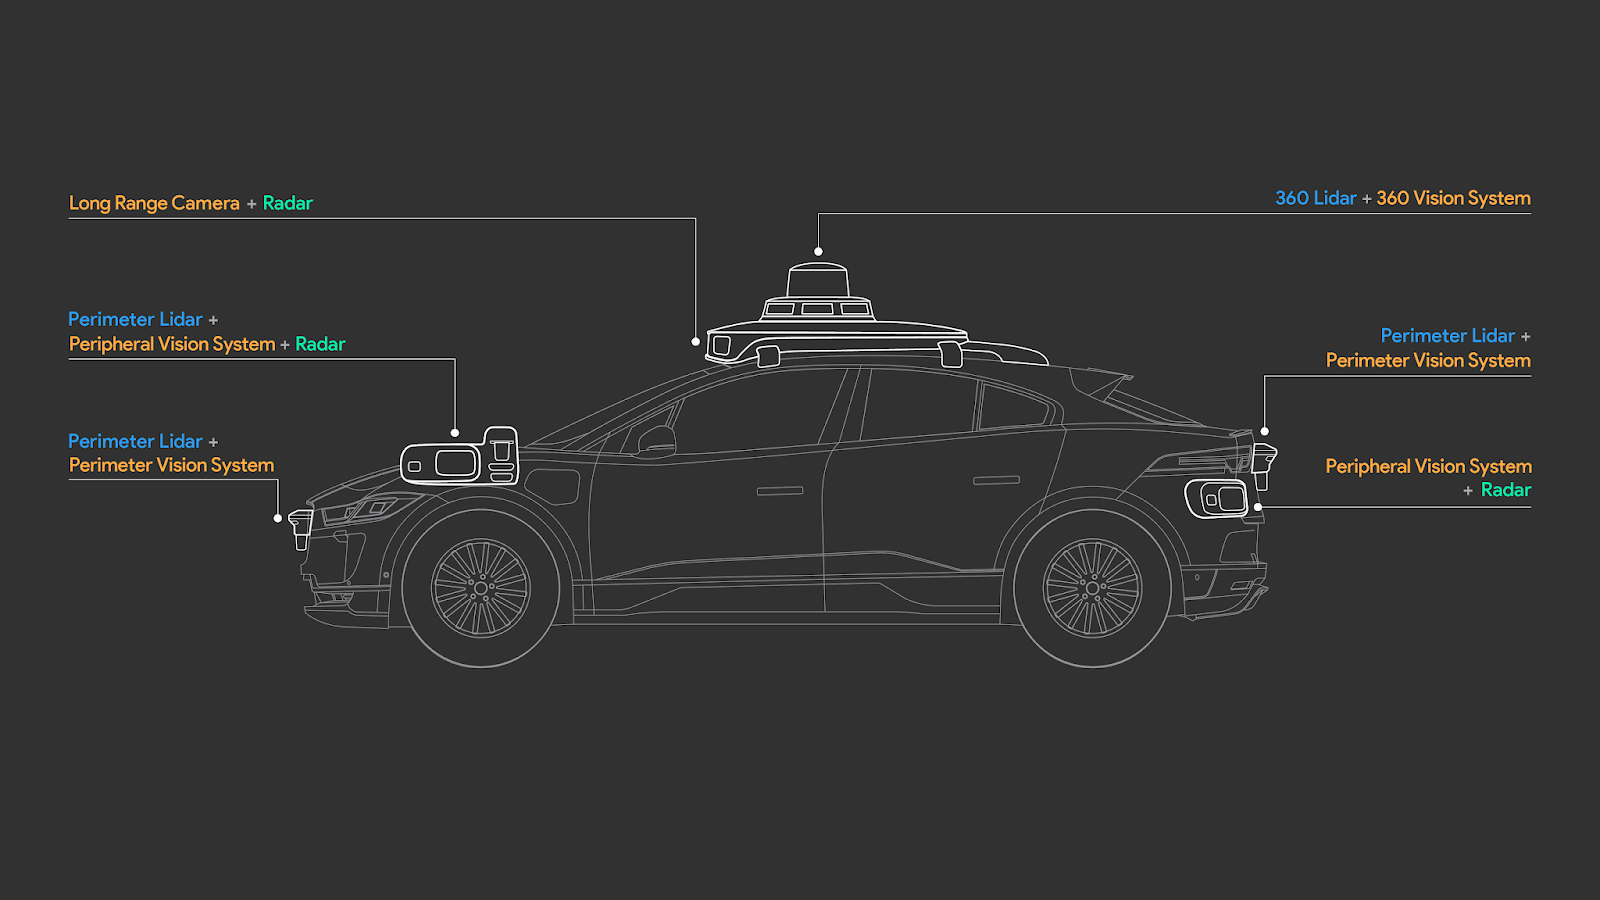
\includegraphics[width=15cm]{resources/figures/waymo_driver_sensors.png}
\caption{Układ czujników systemu Waymo Driver}
\label{WaymoDriverSensors}
\end{center}
\end{figure}

Czujniki LiDAR mają wysoką rozdzielczość i zasięg do 300 metrów. Kamery dają bardzo ostry obraz o dobrej jakości. System widzenia obwodowego działa we współpracy z systemem LiDAR-ów obwodowych (z ang. \textit{perimeter lidars}), dzięki czemu samochód lepiej widzi co się dzieje w jego najbliższym otoczeniu - to pomaga w wielu sytuacjach, na przykład podczas manewrów parkowania. Radary wspomagają pracę czujników LiDAR w trudnych warunkach pogodowych, odznaczają się także wysoką rozdzielczością i zasięgiem rzędu kilkuset metrów.

\subsection{NVIDIA DRIVE}
Firma NVIDIA od dawna inwestuje w rozwój technologii samochodów autonomicznych. Oferowane przez nich rozwiązania noszą nazwę NVIDIA DRIVE \cite{nvidiaDrive:overview}. Są to kompleksowe rozwiązania sprzętowo-programowe, stanowiące bazę do tworzenia autonomicznych pojazdów. NVIDIA prowadzi współpracę z wieloma partnerami działającymi w branży automotive \cite{nvidiaDrive:partners}, a wśród nich są: Audi, Toyota, Volkswagen, Volvo.

Dlaczego NVIDIA DRIVE jest tak wyjątkowe? Ponieważ otwiera ono drogę do zupełnie nowych możliwości dla firm zainteresowanych tematyką jazdy autonomicznej. Firmy te nie potrzebują prowadzić działów badawczo-rozwojowych w celu opracowania własnej technologii, tylko mogą wykupić istniejące rozwiązanie i zintegrować go ze swoim systemem. Jednym ze spektakularnych przypadków użycia NVIDIA DRIVE było szybkie wdrożenie usługi przewozów miejskich, wykonane przez firmę Optimus Ride \cite{nvidiaDrive:optimusRide}.

Rozwiązania oferowane w ramach NVIDIA DRIVE można podzielić na dwie części: sprzętową (hardware) oraz programową (software).

\subsubsection{Rozwiązania sprzętowe}
Sprzęt oferowany w ramach NVIDIA DRIVE tworzy rodzinę platform obliczeniowych o nazwie NVIDIA DRIVE AGX. W skład rodziny wchodzą obecnie dwa modele:
\begin{enumerate*}
\item NVIDIA DRIVE AGX Pegasus \\
Posiada moc obliczeniową 320 TOPS (Tera Operations Per Second), co wciąż czyni go jednym z najszybszych rozwiązań dostępnych na rynku.
Architekturę oparto na dwóch procesorach NVIDIA Xavier i dwóch układach graficznych TensorCore. Bardzo efektywny energetycznie, pobiera niewielką ilość prądu w stosunku do wydajności jaką posiada. Może zostać wykorzystany przy tworzeniu w pełni autonomicznych systemów jazdy, co oznacza że pedały i kierownica nie są wymagane. \\

\begin{figure}[h]
\begin{center}
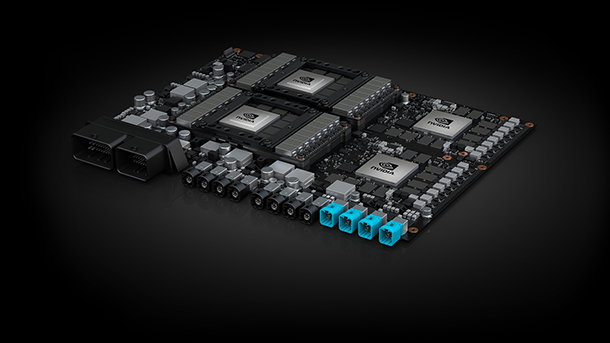
\includegraphics[width=15cm]{resources/figures/nv-drive-pegasus.jpg}
\caption{NVIDIA DRIVE AGX Pegasus}
\end{center}
\end{figure}
\newpage
\item NVIDIA DRIVE AGX Xavier \\
Mniejszy od Pegasusa, charakteryzuje się też mniejszą mocą obliczeniową oscylującą w granicach 30 TOPS. Zużycie energii jest jednak bardzo niskie, ponieważ wynosi tylko 30 watów. Ta platforma obliczeniowa jest za słaba żeby obsłużyć w pełni autonomiczne systemy jazdy, ale dobrze sobie radzi przy częściowej automatyzacji sterowania. \\

\begin{figure}[h]
\begin{center}
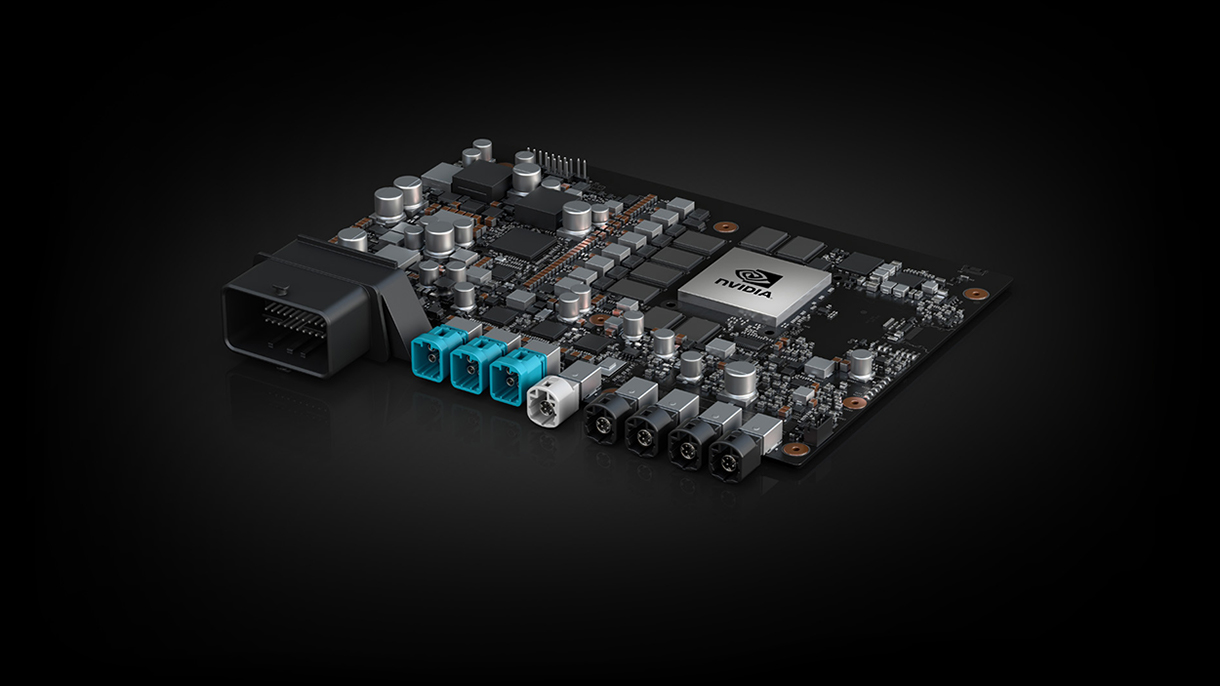
\includegraphics[width=15cm]{resources/figures/nv-drive-xavier.jpg}
\caption{NVIDIA DRIVE AGX Xavier}
\end{center}
\end{figure}
\end{enumerate*}

Oprócz tego w skład rozwiązań sprzętowych wchodzi także NVIDIA DRIVE Hyperion, czyli najbardziej kompleksowe rozwiązanie oferowane przez firmę NVIDIA \cite{nvidiaDrive:hyperion}. W skład tego rozwiązania wchodzi platforma obliczeniowa (Xavier lub Pegasus), zestaw czujników oraz oprogramowanie sterujące.

\subsubsection{Oprogramowanie NVIDIA DRIVE}
Oprogramowanie NVIDIA DRIVE składa się z następujących modułów \cite{nvidiaDrive:sdk}:
\begin{enumerate*}
\item DRIVE OS \\
Podstawowy stos oprogramowania składający się z systemu operacyjnego czasu rzeczywistego (RTOS), modułu NVIDIA Hypervisor, bibliotek NVIDIA CUDA oraz NVIDIA TensorRT \cite{nvidia:tensorRt} a także innych modułów umożliwiających dostęp do zasobów sprzętowych. DRIVE OS zapewnia bezpieczne i stabilne środowisko wykonawcze dla uruchamianych aplikacji. Najważniejsze cechy modułu DRIVE OS:
\begin{itemize*}
\item Wieloużytkownikowy, 64-bitowy system operacyjny;
\item Platforma CUDA dla równoległych obliczeń;
\item API NvMedia dla akcelerowanych sprzętowo multimediów oraz przetwarzania danych z kamery;
\item API graficzne: OpenGL, OpenGL ES, EGL z rozszerzeniami EGLStream;
\item Biblioteki głębokiego uczenia maszynowego: TensorRT, cuDNN.
\end{itemize*}
\item DriveWorks \\
Zestaw do tworzenia oprogramowania (SDK) pozwalający programistom na implementację oprogramowania dla samochodów autonomicznych poprzez dostarczanie zbioru przydatnych bibliotek i narzędzi deweloperskich. Zestaw ten został zaprojektowany z myślą o maksymalnym wykorzystaniu możliwości sprzętowych komputera, ze szczególnym uwzględnieniem jego przepustowości. \\
Najważniejsze cechy modułu DriveWorks:
\begin{itemize*}
\item Efektywne wykorzystanie wszystkich dostępnych procesorów;
\item Optymalizacja formatu danych komunikacji pomiędzy silnikami sprzętowymi;
\item Ograniczenie kopiowania danych do niezbędnego minimum;
\item Wykorzystanie bardzo wydajnych algorytmów.
\end{itemize*}
\item DRIVE AV \\
Dostarcza modułów percepcji, mapowania oraz planowania. Percepcja pozwala na wykrywanie i śledzenie obiektów rejestrowanych przez czujniki oraz obliczanie odległości pomiędzy nimi. Mapowanie zbiera i przypisuje zanonimizowane dane od użytkowników platformy NVIDIA DRIVE Hyperion w celu uzyskania bezpiecznego, niezawodnego i aktualnego pokrycia map w jakości HD. Planowanie służy m.in. do wyznaczania ścieżek przejazdu dla samochodu.
\item DRIVE IX \\
Otwartoźródłowy moduł oprogramowania do obsługi czujników wnętrza kabiny. Jest niezbędny do wprowadzenia innowacyjnych rozwiązań kokpitu AI, takich jak monitorowanie zachowań kierowcy oraz interakcja głosowa człowieka z maszyną.
\end{enumerate*}
Moduły oprogramowania NVIDIA DRIVE zostały zaprezentowane na rysunku \ref{NvidiaDriveSDK}.
\newpage
\begin{figure}[h]
\begin{center}
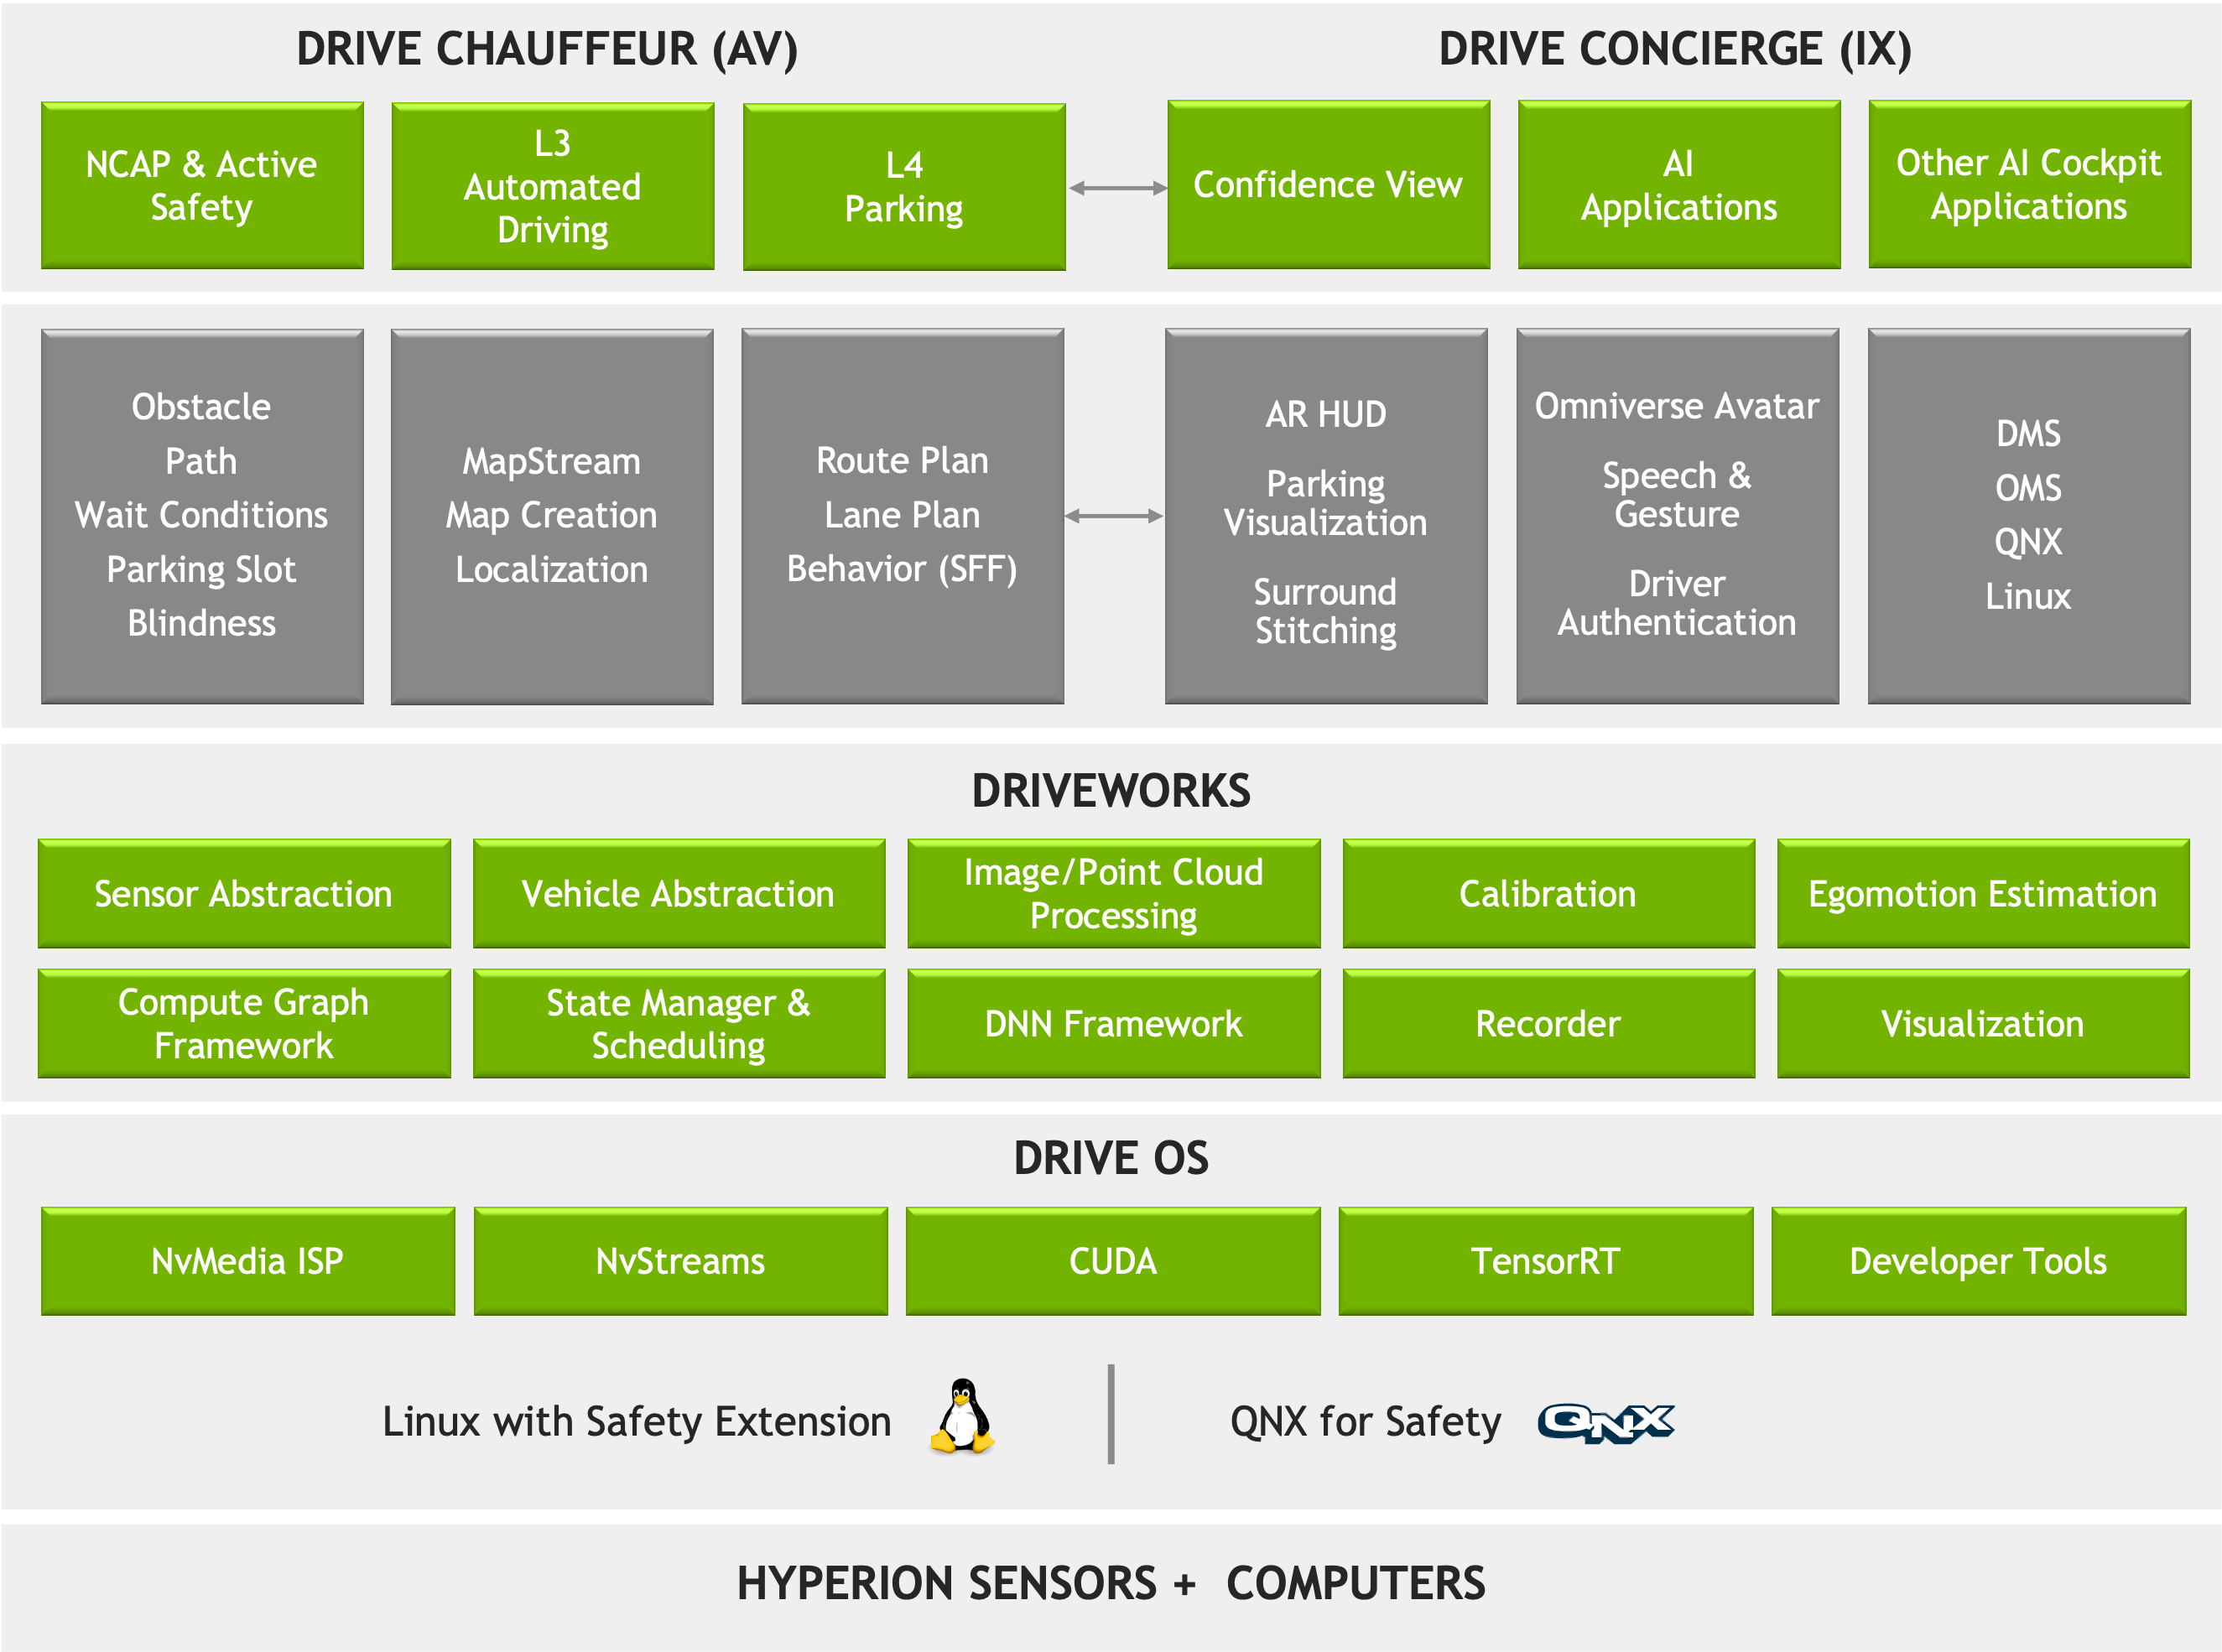
\includegraphics[width=15cm]{resources/figures/nv-drive-sdk.png}
\caption{Moduły oprogramowania NVIDIA DRIVE}
\label{NvidiaDriveSDK}
\end{center}
\end{figure}

\subsection{Tesla Autopilot}
Firma Tesla zasłynęła produkcją swoich samochodów elektrycznych. Opracowała również zaawansowany system wspomagania jazdy, noszący nazwę \textbf{Tesla Autopilot} \cite{tesla:autopilotOverview}. System ten został stworzony w celu zwiększenia bezpieczeństwa oraz komfortu podróżowania kierowcy, pasażerów oraz innych uczestników ruchu drogowego. Każdy nowy samochód Tesli wyposażony jest w osiem kamer, a samochody sprzedawane poza Ameryką Północną są również wyposażone w zestaw czujników radarowych. Autopilot nie zapewnia pełnej autonomii samochodu, dlatego też kierowca musi zachować czujność podczas jazdy i być gotów przejąć kontrolę nad sterowaniem gdy zajdzie taka potrzeba.

W skład Autopilota wchodzą następujące funkcje:
\begin{enumerate*}
\item \textbf{Traffic-Aware Cruise Control} - dopasowuje prędkość samochodu do otaczającego ruchu ulicznego;
\item \textbf{Autosteer} - wspomaga kierowanie na drodze posiadającej wyraźnie oznaczone pasy ruchu oraz wykorzystuje aktywny tempomat, który uwzględnia ruch drogowy wokół samochodu.
\end{enumerate*}

Tesla oferuje również pakiet rozszerzeń o nazwie \textbf{Full Self-Driving Capability}, który wzbogaca Autopilota o takie funkcje jak:
\vspace{-0.25cm}
\begin{enumerate*}
\item \textbf{Navigate on Autopilot} - umożliwia półautonomiczną jazdę po autostradzie.
\item \textbf{Auto Lane Change} - pomaga w zmianie pasa ruchu na autostradzie, gdy jest włączona funkcja \textbf{Autosteer}.
\item \textbf{Autopark} - pomaga zaparkować samochód równolegle lub prostopadle.
\item \textbf{Summon} - wprowadza oraz wyprowadza samochód z ciasnej przestrzeni za pomocą aplikacji mobilnej.
\item \textbf{Smart Summon} - samochód nawiguje po skomplikowanych obiektach typu place parkingowe, aby odnaleźć kierowcę i podjechać do niego.
\item \textbf{Stop Sign and Traffic Light Control} - pierwsza funkcja przeznaczona do użytku w ruchu miejskim. Pojazdy Tesli wyposażone w tę funkcję potrafią reagować na znaki stop oraz sygnalizację świetlną. Przy dojeżdżaniu do skrzyżowania ze światłami samochód zwalnia (nawet mając zielone), a kierowca musi nacisnąć pedał przyspieszenia aby samochód mógł kontynuować jazdę w trybie automatycznym.
\end{enumerate*}

Jakby tego było mało, to samochody Tesli są wyposażone w zestaw aktywnych funkcji bezpieczeństwa:
\vspace{-0.25cm}
\begin{enumerate*}
\item \textbf{Automatic Emergency Braking} - wykrywa przeszkody, w które samochód mógłby uderzyć i odpowiednio do sytuacji uruchamia hamulce;
\item \textbf{Forward Collision Warning} - ostrzega przed nadciągającą kolizją z wolniej poruszającymi się lub nieruchomymi samochodami;
\item \textbf{Side Collision Warning} - ostrzega przed potencjalną kolizją z obiektami rozmieszczonymi wokół samochodu;
\item \textbf{Obstacle Aware Acceleration} - automatycznie zmniejsza przyspieszenie samochodu po wykryciu przeszkody podczas jazdy z małą prędkością;
\item \textbf{Blind Spot Monitoring} - ostrzega przed obiektami w martwym polu, gdy samochód wykonuje manewr zmiany pasa;
\item \textbf{Lane Departure Avoidance} - stosuje manewry korygujące w celu utrzymania się na swoim pasie ruchu;
\item \textbf{Emergency Lane Departure Avoidance} - przywraca pojazd z powrotem na swój pas ruchu, gdy wykrywa że samochód zjeżdża ze swojego pasa i może dojść do kolizji na drodze.
\end{enumerate*}

\subsubsection{Tesla Vision}
Tesla jest obecnie liderem na rynku pod względem rozwoju technologii wykorzystania kamer w samochodach autonomicznych. Ich system o nazwie 
\textbf{Tesla Vision} to nowa wersja systemu \textbf{Tesla Autopilot}, w której całą percepcję oparto tylko na jednym typie czujnika: kamerze. Począwszy od maja 2021, system ten jest montowany w samochodach Tesli sprzedawanych w Ameryce Północnej \cite{tesla:transToVision}.

Pomysł całkowitej rezygnacji z radarów oraz LiDAR-ów wzbudził wiele kontrowersji w środowisku osób zainteresowanych rozwojem technologii samochodów autonomicznych. W dość obszernym artykule \cite{torchinsky:teslaRemoveRadar} z maja 2021 roku, autor wysuwa szereg trafnych argumentów przeciwko decyzji Tesli o rezygnacji z montowania radarów w niektórych ich modelach. Radary doskonale uzupełniają dane z kamer, zwłaszcza w sytuacji kiepskiej widoczności na drodze. Z radarami łatwiej jest generować trójwymiarową reprezentację otoczenia samochodu, ponieważ uzyskujemy ją bezpośrednio z odczytów radaru (w przeciwieństwie do obrazu z kamery, gdzie informacja o głębi musi zostać obliczona przez oprogramowanie pojazdu). Sygnał z radarów jest w stanie prześlizgnąć się i wrócić pod samochodami jadącymi bezpośrednio przed samochodem autonomicznym, dzięki czemu samochód może zareagować z większym wyprzedzeniem i uniknąć kolizji, do której doszłoby w innym wypadku.

Autora nie przekonują argumenty typu ,,\textit{człowiek też nie ma radarów i jakoś sobie radzi z prowadzeniem samochodu}'', ponieważ ignorują one fundamentalny problem, jaki przeszkadza w osiągnięciu pełnej autonomii pojazdu: nasze oprogramowanie wciąż jest bardzo dalekie od tego, co potrafi ludzki mózg. Dotyczy to zarówno umiejętności sprawnego interpretowania obrazów, jak również logicznego rozumowania oraz zdolności adaptacji do nowego środowiska i radzenia sobie w niestandardowych scenariuszach drogowych. Na każdym z tych pól oprogramowanie wykazuje poważne braki i niedociągnięcia w stosunku do możliwości człowieka. Skoro Tesla nie wprowadziła żadnej rewolucji w tym zakresie, to pozbycie się radarów dających cenne źródło informacji należy uznać za regresję w możliwościach systemu. Zwłaszcza, że nie wprowadzono żadnej redundancji w postaci dodatkowych kamer, dlatego też przy awarii chociaż jednej z nich lub nawet zasłonięciu soczewki (np. z powodu zalegającego śniegu lub ptasich odchodów) percepcja samochodu ulega znaczącemu pogorszeniu.

Pomimo powyższych zastrzeżeń wygląda na to, że Tesla nieustannie doskonali swój produkt i wraz z kolejnymi aktualizacjami oprogramowania ich samochody radzą sobie coraz lepiej - również w trudnych warunkach pogodowych, co zostało opisane w artykule \cite{klender:teslaOnHeavyRain}. Autor przedstawił odczucia jednego z użytkowników samochodu Tesli, który zauważał postępującą poprawę zachowania samochodu podczas jazdy w intensywnym deszczu. Poprawa ta następowała (w mniejszym lub większym stopniu) po każdej aktualizacji oprogramowania i objawiała się mniejszym i mniej gwałtownym wytracaniem prędkości pojazdu.

Podczas konferencji CVPR odbytej w 2021 roku, Andrej Karpathy (szef działu AI w Tesli) wyjaśnił dlaczego Tesla zrezygnowała z wykorzystania czujników LiDAR w swoich samochodach \cite{dickson:teslaDontNeedLidar}. Karpathy wskazał między innymi na problem przygotowania i utrzymania dokładnych i szczegółowych map 3D terenu, po którym ma się poruszać samochód wyposażony w czujniki LiDAR. ,,\textit{Musisz wstępnie zmapować środowisko za pomocą LiDAR-u, a następnie stworzyć mapę w wysokiej rozdzielczości i wstawić tam wszystkie pasy i sygnalizacje świetlne}'' - powiedział Karpathy. Dodał również: ,,\textit{Zbieranie, budowanie i utrzymywanie map LiDAR-owych w wysokiej rozdzielczości jest nieskalowalne. Bardzo trudno utrzymać tę infrastrukturę w stanie aktualnym}''. Samochody Tesli nie potrzebują mieć ręcznie przygotowanych map 3D, ponieważ same potrafią wygenerować sobie takie mapy. ,,\textit{Wszystko co się dzieje, dzieje się po raz pierwszy w samochodzie, na podstawie nagrań z ośmiu kamer otaczających samochód}'' - stwierdził Andrej Karpathy. Samochód musi samodzielnie rozpoznać otoczenie, wykryć i zinterpretować wszystkie elementy infrastruktury drogowej oraz ocenić, które z nich są dla niego istotne. Wszystko to bez jakiejkolwiek wcześniejszej informacji na temat drogi, po której samochód będzie się przemieszczać.

\subsubsection{Platforma sprzętowa}
Dodatkowym warunkiem, jaki musi spełniać samochód autonomiczny, jest maksymalny dopuszczalny czas obliczeń podczas jazdy samochodem. Wszystko musi odbywać się w czasie rzeczywistym, a zbyt wielkie opóźnienia w przetwarzaniu danych mogłyby doprowadzić do wystąpienia niebezpiecznej sytuacji na drodze. Na szczęście Tesla dysponuje bardzo dobrym sprzętem, opracowanym we współpracy z firmą Samsung \cite{wiggers:teslaDrivingChip}. Nosi on nazwę \textbf{Full Self-Driving Computer} (FSD) i w momencie swojej premiery w 2019 roku był określany jako ,,\textit{najbardziej zaawansowany komputer przeznaczony dla jazdy autonomicznej}''.

Chipset Samsunga osiąga wydajność 144 TOPS i składa się z dwóch redundantnych, niezależnych pakietów - każdy z nich dysponuje własną pamięcią DRAM, układami pamięci flash oraz zasilaniem. ,,\textit{Każdy z pakietów uruchamia i utrzymuje własną instancję systemu operacyjnego}'' - mówi Pete Bannon, projektant układów scalonych pracujący dla Tesli. Dwa pakiety niezależnie od siebie dokonują obliczeń akcji do wykonania, a następnie wymieniają się ze sobą wynikami obliczeń. Żadna akcja nie zostanie zlecona do wykonania kontrolerom samochodu do czasu jej uzgodnienia i zatwierdzenia przez obydwa pakiety. Układ zachowuje swoją zdolność działania także wtedy, gdy jeden z pakietów (lub któraś z jego części) ulegnie awarii. Elon Musk stwierdził, że: ,,\textit{nawet jeśli część układu ulegnie awarii, samochód wciąż może kontynuować jazdę}''.

FSD składa się z 6 miliardów tranzystorów i 250 milionów bramek logicznych. Jego moduły pamięci LPDDR4 RAM zapewniają przepustowość 68 GB/s, a zintegrowane procesory przetwarzania obrazów potrafią pracować z prędkością do 1 gigapiksela na sekundę. Dodatkowo w zestawie są dwa akceleratory sieci neuronowych, taktowane z częstotliwością 2 GHz i wyposażone w 32 MB pamięci SRAM. Akceleratory mogą dodawać macierze oraz przetwarzać do 1 TB danych na sekundę, a ich wydajność wynosi 36 TOPS dla każdego z nich (czyli łącznie 72 TOPS). Innym ważnym komponentem jest wbudowany układ zabezpieczający, którego zadaniem jest blokowanie kodu nieposiadającego podpisu kryptograficznego Tesli.

Podczas testów zamkniętych, przeprowadzonych przez firmę Tesla, okazało się że komputer FSD jest w stanie przetwarzać 2300 klatek na sekundę - podczas gdy poprzednia generacja komputera osiągała zaledwie 110 klatek na sekundę. \\

\begin{figure}[h]
\begin{center}
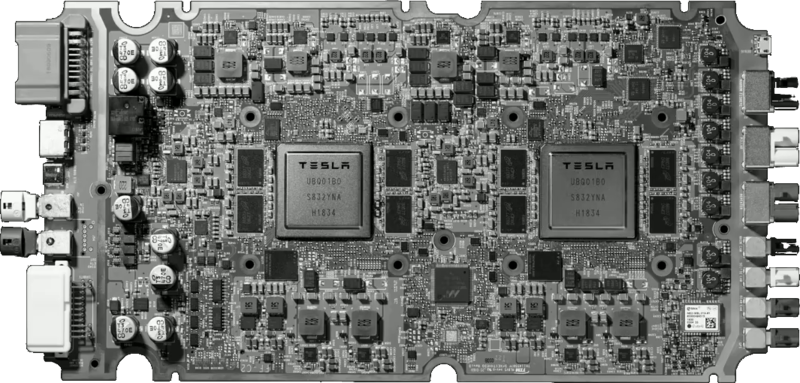
\includegraphics[width=15cm]{resources/figures/tesla_fsd.png}
\caption{Komputer Tesla FSD}
\end{center}
\end{figure}

\vspace{-0.7cm}
\subsubsection{Podsumowanie}
Tesla Autopilot to niezwykle ciekawy i wyróżniający się na tle konkurencji projekt. Przedstawiciele Tesli wnieśli ważny głos do dyskusji nad rozwojem technologii samochodów autonomicznych, zwłaszcza w konteście wykorzystania obrazu z kamery jako głównego źródła danych dla modelu percepcji pojazdu. Wkład firmy w rozwój technologii jest bezcenny, nawet jeśli zastosowane podejście okaże się ślepym zaułkiem w drodze do osiągnięcia w pełni autonomicznego systemu sterowania samochodem.
\chapter{Konwolucyjne sieci neuronowe}
\chapter{Projekt systemu i opis narzędzi}
\label{DesignSystemChapter}
W poniższym rozdziale zostaną zaprezentowane kluczowe decyzje projektowe oraz założenia, jakie zostały przyjęte w toku prac nad implementacją systemu. Oprócz tego zostanie również przedstawiony opis narzędzi, które zostały wykorzystane do stworzenia aplikacji.

\section{Projekt systemu}
W fazie projektowania należy zdefiniować główne założenia projektowe oraz odpowiednio zaprojektować architekturę systemu. Podsumowując wyniki uzyskane w tej fazie, zdecydowałem się rozpatrzeć trzy najważniejsze zagadnienia:
\begin{enumerate*}
\item Definicja \textbf{rozwiązywanego problemu},
\item Lista \textbf{celów i założeń systemu},
\item \textbf{Architektura systemu}, rozpatrywana na najwyższym poziomie abstrakcji.
\end{enumerate*}

\subsection{Definicja rozwiązywanego problemu}
Zaprojektowany system powinien rozwiązywać problem treningu agentów sterujących samochodem w środowisku symulacji. Samochód powinien pokonywać wyznaczony tor wyścigowy w możliwie najkrótszym czasie. Agenci odbierają informacje o swoim aktualnym położeniu dzięki obrazowi z jednej lub kilku kamer doczepionych do samochodu. W odpowiedzi na te informacje, do środowiska symulacji wysyłane są żądania podjęcia określonych zachowań, np. zmiany poziomu wciśnięcia pedału hamulca. Ponadto, środowisko symulacji na bieżąco przyznaje agentom nagrody i kary w zależności od tego, jak dobrze (lub źle) agent radzi sobie z postawionym zadaniem. Odpowiedni system kar i nagród jest kluczowy dla osiągnięcia zadowalających wyników treningu.

Agentami są konwolucyjne sieci neuronowe, a ich parametry są dostrajane przy użyciu metody uczenia maszynowego zwanej \textbf{uczeniem ze wzmocnieniem} (z ang. \textit{reinforcement learning}) \cite{deepRL:guide}.

\subsection{Cele i założenia}
\begin{enumerate*}
\item Stworzony system powinien być możliwie prosty w obsłudze.
\item Wytrenowane modele powinny być zapisywane do pliku o ustalonym formacie. Format pliku musi być rozpoznawany i obsługiwany przez aplikację.
\item Dane konfiguracyjne powinny być dostarczane z zewnętrznego pliku o ustalonym formacie.
\item System powinien zapisywać przebieg treningu sieci neuronowych w postaci plików dziennika. Pliki te powinny zawierać informacje ułatwiające późniejszą analizę treningu.
\item System powinien posiadać możliwość podglądu ,,na żywo'' postępów treningu sieci podczas jego trwania.
\end{enumerate*}

\subsection{Architektura systemu}
\label{SoftwareArchSection}
System składa się z dwóch zasadniczych modułów: Środowiska Uczenia oraz narzędzia \texttt{mlagents\_learn}. Moduły komunikują się ze sobą za pośrednictwem mechanizmu komunikacji dostarczanego przez zestaw Unity ML-Agents. Wizualizacja architektury systemu została przedstawiona na rysunku \ref{SystemArchitecture}, a więcej informacji na temat każdego z modułów można uzyskać w rozdziale \ref{ImplementationChapter}-tym, poświęconym opisowi implementacji systemu. \\

\begin{figure}[h]
\begin{center}

\includegraphics[width=15cm]{resources/figures/system_architecture.png}
\caption{Wizualizacja architektury systemu.}
\label{SystemArchitecture}
\end{center}
\end{figure}

\section{Opis narzędzi}
W tej sekcji zamieszczam opis narzędzi wykorzystanych do implementacji systemu.
\subsection{Unity}
Multiplatformowy silnik gier 2D i 3D \cite{unity:opis}, napisany w językach C/C++.
Skrypty silnika należy pisać w języku C\#.
Gry tworzone na silniku Unity mogą być uruchamiane na bardzo wielu platformach sprzętowych i systemowych \cite{unity:buildTargets}:
\begin{enumerate*}
\item Komputery osobiste (PC):
\begin{itemize*}
\item Windows,
\item Linux,
\item Mac OS X;
\end{itemize*}
\item Urządzenia mobilne (smartfony):
\begin{itemize*}
\item Android,
\item iOS;
\end{itemize*}
\item Konsole do gier:
\begin{itemize*}
\item PlayStation 4,
\item PlayStation 5,
\item Xbox One,
\item Nintendo Switch;
\end{itemize*}
\item i wiele innych.
\end{enumerate*}

Unity posiada bardzo atrakcyjne warunki licencyjne - niemal wszystkie funkcje silnika są dostępne za darmo dla twórców nieprzekraczających 100 tysięcy dolarów rocznego dochodu.

W Unity powstało wiele popularnych gier, takich jak:
\begin{enumerate*}
\item Pokémon Go,
\item Hearthstone: Heroes of Warcraft,
\item Firewatch,
\item The Forest,
\item Car Mechanic Simulator,
\item Gwint: Wiedźmińska Gra Karciana,
\item Syberia 3,
\item i wiele innych.
\end{enumerate*}

Warto również wspomnieć o module Unity Asset Store, który zezwala na wykorzystanie płatnych i darmowych komponentów, takich jak tekstury, modele czy skrypty.

\subsection{C\#}
Język programowania stworzony przez firmę Microsoft jako konkurencja dla Javy \cite{csharp:opis}. Jest wysokopoziomowym, obiektowym językiem programowania, ściśle zintegrowanym z platformą .NET (pełniącą rolę frameworka oraz środowiska uruchomieniowego). Charakteryzuje się silnym, statycznym typowaniem. C\# pozwala na tworzenie aplikacji desktopowych (Windows, Linux, MacOS), webowych (poprzez użycie frameworka ASP.NET) oraz multiplatformowych aplikacji mobilnych (poprzez wykorzystanie narzędzia Xamarin). Obecnie jest to jeden z najpopularniejszych języków programowania.

\subsection{Unity ML-Agents}
\label{UnityMlSection}
Otwartoźródłowy zestaw narzędzi przeznaczony dla silnika Unity 3D \cite{unitymla:overview}. Został stworzony w celu ułatwienia treningu sieci neuronowych w środowiskach symulowanych komputerowo. Sieci neuronowe mogą być trenowane przy użyciu jednej z kilku możliwych metod uczenia maszynowego:
\begin{enumerate*}
\item Uczenie ze wzmocnieniem (z ang. \textit{reinforcement learning}) \cite{deepRL:guide}:
\begin{itemize*}
\item wykorzystując algorytm PPO \cite{ppo:opis};
\item wykorzystując algorytm SAC \cite{sac:opis};
\end{itemize*}
\item Uczenie przez imitację (z ang. \textit{imitation learning}) \cite{imitationLearning:article},
\item Neuroewolucja \cite{neuroevolution:primer},
\item Inna metoda uczenia maszynowego - zdefiniowana przez użytkownika.
\end{enumerate*}

Zestaw Unity ML-Agents składa się z pięciu podstawowych komponentów:
\begin{enumerate*}
\item Środowisko Uczenia (z ang. \textit{Learning Environment}) - obejmuje scenę Unity oraz wszystkie obiekty znajdujące się na niej. Scena Unity dostarcza środowisko do generowania obserwacji, wykonywania działań i uczenia się.
\item Niskopoziomowe API Pythona (z ang. \textit{Python Low-Level API}) \cite{unitymla:pythonapi} - zawiera niskopoziomowy interfejs programistyczny służący do komunikacji ze Środowiskiem Uczenia. API Pythona nie jest częścią silnika Unity, ale istnieje jako osobny byt komunikujący się z Unity dzięki Zewnętrznemu Komunikatorowi. API jest zaimplementowane w języku Python i zawarte w pakiecie o nazwie \texttt{mlagents\_envs}.
\item Zewnętrzny Komunikator (z ang. \textit{External Communicator}) - łączy Środowisko Uczenia z Niskopoziomowym API Pythona.
\item Trenerzy Pythona (z ang. \textit{Python Trainers}) - zawiera wszystkie algorytmy uczenia maszynowego dostarczane przez Unity ML-Agents. Algorytmy zaimplementowane są w języku Python i należą do pakietu o nazwie \texttt{mlagents}. Pakiet udostępnia narzędzie wiersza poleceń o nazwie \texttt{mlagents-learn}, które obsługuje wszystkie metody treningu i opcje opisane powyżej.
\item Gym Wrapper - opisany w dokumentacji zestawu \cite{unitymla:gymWrapper}. Mało istotny dla dalszych rozważań.
\end{enumerate*}

Rysunek \ref{UnityMlaComponents} przedstawia diagram opisanych powyżej komponentów zestawu Unity ML-Agents. Gym Wrapper został na nim pominięty.

\begin{figure}[h]
\begin{center}
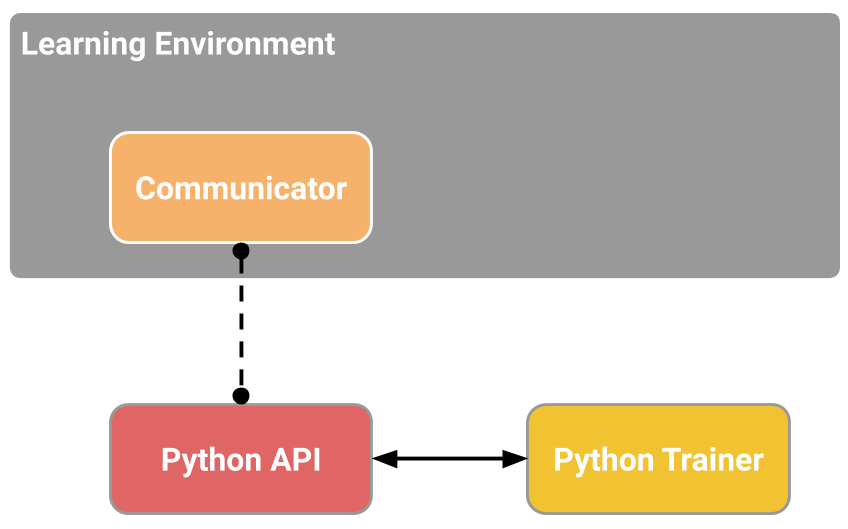
\includegraphics[width=15cm]{resources/figures/learning_environment_basic.png}
\caption{Diagram komponentów Unity ML-Agents}
\source{https://github.com/Unity-Technologies/ml-agents/blob/release_19_docs/docs/ML-Agents-Overview.md}
\label{UnityMlaComponents}
\end{center}
\end{figure}

Poprawnie skonfigurowane Środowisko Uczenia musi zawierać następujące elementy:
\begin{enumerate*}
\item Co najmniej jednego Agenta (z ang. \textit{Agent}). Agent to komponent dołączany do obiektu klasy \texttt{GameObject}, umiejscowionego na scenie Unity. Każdy Agent jest instancją klasy dziedziczącej po klasie \texttt{Agent}. Agent zajmuje się generowaniem Obserwacji, wykonywaniem Akcji oraz przydzielaniem Nagród.
\item Co najmniej jednego Zachowania (z ang. \textit{Behavior}). Zachowanie definiuje określone atrybuty Agenta, takie jak liczba i rodzaj wykonywanych Akcji. Każde Zachowanie jest jednoznacznie identyfikowane poprzez pole \texttt{Behavior Name}. \\
Istnieją trzy rodzaje Zachowań:
\begin{itemize*}
\item Zachowanie Uczące (z ang. \textit{Learning Behavior}) - Zachowanie którego Agent musi się wyuczyć. Tego Zachowania używamy podczas treningu sieci neuronowych;
\item Zachowanie Heurystyczne (z ang. \textit{Heuristic Behavior}) - Zachowanie zdefiniowane przez reguły zapisane bezpośrednio w kodzie źródłowym. Przydatne m.in. przy testowaniu nowego Środowiska Uczenia przed rozpoczęciem treningu sieci.
\item Zachowanie Wnioskujące (z ang. \textit{Inference Behavior}) - Zachowanie wykorzystujące wytrenowany model sieci neuronowej. W gruncie rzeczy, Zachowanie Uczące po skończonym treningu sieci neuronowej zmienia się w Zachowanie Wnioskujące.
\end{itemize*}
\end{enumerate*}

\begin{figure}[h]
\begin{center}
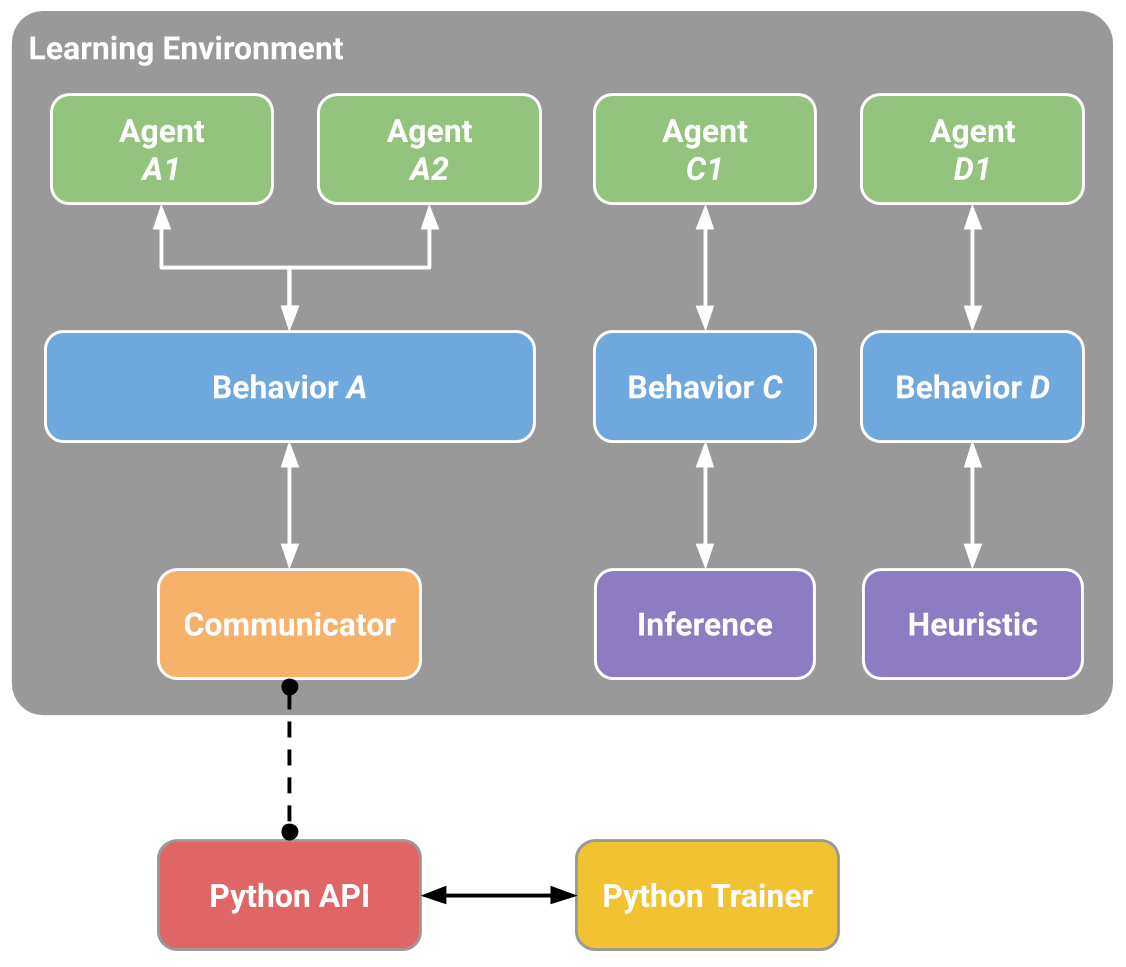
\includegraphics[width=15cm]{resources/figures/learning_environment_example.png}
\caption{Przykład relacji Agentów z Zachowaniami w Środowisku Uczenia}
\source{https://github.com/Unity-Technologies/ml-agents/blob/release_19_docs/docs/ML-Agents-Overview.md}
\label{UnityMlaExample}
\end{center}
\end{figure}

Każdy Agent musi być powiązany z dokładnie jednym Zachowaniem, a Zachowanie może być połączone z więcej niż jednym Agentem. Agenci działający wedle tej samej logiki powinni być powiązani z tym samym Zachowaniem. To wcale nie oznacza, że wszyscy Agenci powiązani z tym samym Zachowaniem muszą współdzielić ze sobą te same Obserwacje, Akcje i Nagrody.

Rysunek \ref{UnityMlaExample} przedstawia przykładowy diagram zależności Agentów z Zachowaniami w Środowisku Uczenia. Agenci \texttt{A1} i \texttt{A2} są podłączeni do Zachowania Uczącego. Agenci \texttt{C1} i \texttt{D1} są podłączeni odpowiednio do Zachowania Wnioskującego i Heurystycznego.

Opisując narzędzie Unity ML-Agents, należałoby również wspomnieć kilka słów o samym Agencie. Każdy Agent wykonuje cyklicznie trzy czynności: generuje Obserwacje, wykonuje zlecone Akcje i oblicza wartość Nagrody. Omówmy każdy z tych elementów:
\begin{enumerate*}
\item Obserwacje (z ang. \textit{Observations}) - zestaw danych wejściowych, niezbędnych do wykonania zleconego Agentowi zadania. Obserwacje mogą być generowane na kilka sposobów:
\begin{itemize*}
\item Nadpisanie metody \texttt{Agent.CollectObservations()} i przesłanie obserwacji do dostarczonego (przez parametr metody) obiektu klasy \texttt{VectorSensor}. Ten sposób najlepiej wykorzystać do aspektów środowiska które można opisać numerycznie i niewizualnie.
\item Dodanie atrybutu \texttt{[Observable]} do pól i właściwości Agenta. Atrybut \\ \texttt{[Observable]} wspiera obecnie podstawowe typy danych (takie jak  \texttt{int}, \texttt{float} czy \texttt{bool}), jak również klasy \texttt{Vector2}, \texttt{Vector3}, \texttt{Vector4}, \texttt{Quaternion} oraz typy enumeracyjne.
\item Implementacja interfejsu \texttt{ISensor}, korzystając z \texttt{SensorComponent} dołączanego do Agenta. Obecnie istnieje kilka implementacji komponentu \texttt{SensorComponent} dostarczanych przez API zestawu Unity ML-Agents. Najważniejsze z nich to:
\begin{itemize*}
\item \texttt{CameraSensorComponent} - używa obrazów z kamery jako obserwacji;
\item \texttt{RenderTextureSensorComponent} - używa zawartości \texttt{RenderTexture} \cite{unity:renderTexture} jako obserwacji;
\item \texttt{RayPerceptionSensorComponent} - używa informacji z zestawu promieni (z ang. \textit{ray casts}) jako obserwacji.
\end{itemize*}
\end{itemize*}
\item Akcje (z ang. \textit{Actions}) - instrukcje zachowań, które Agent powinien wykonać. Istnieją dwa typy Akcji - Ciągłe (z ang. \textit{Continuous}) oraz Nieciągłe (z ang. \textit{Discrete}). Wszystkie Akcje muszą być zdefiniowane w metodzie \texttt{OnActionReceived()}. Akcje Ciągłe to wartości ze zbioru liczb rzeczywistych, podczas gdy Akcje Nieciągłe są wartościami całkowitymi.
\item Nagrody (z ang. \textit{Rewards}) - informacja zwrotna, pozwalająca ocenić jak dobre (lub złe) są Akcje wykonywane obecnie przez Agenta. System Nagród jest najważniejszym elementem w uczeniu ze wzmocnieniem, ponieważ sposób jego skonstruowania ma decydujący wpływ na to, czy trening sieci neuronowej się powiedzie.
\end{enumerate*}

\subsection{Vehicle Physics Pro}
\label{VppSection}
Zaawansowany zestaw do symulacji pojazdów dla silnika Unity 3D. VPP zapewnia wydajny, w pełni realistyczny i dokładny model dynamiki dla niemal każdego typu pojazdu i konfiguracji. W skład zestawu wchodzą m.in. \cite{vpp:features}:
\begin{enumerate*}
\item Wierne odwzorowanie pracy podzespołów pojazdu, obejmujące m.in.:
\begin{itemize*}
\item pracę silnika (spalinowego lub elektrycznego),
\item pracę skrzyni biegów (manualnej lub automatycznej),
\item pracę układu kierowniczego;
\end{itemize*}
\item Symulacja systemów wspomagania jazdy, w tym:
\begin{itemize*}
\item ABS (Anti-lock Braking System),
\item TCS (Traction Control System),
\item ESC (Electronic Stability Control);
\end{itemize*}
\item Liczne rozszerzenia i dodatki, takie jak:
\begin{itemize*}
\item efekty wizualne (np. animacja deski rozdzielczej),
\item efekty dźwiękowe (np. dźwięk silnika),
\item zaawansowana diagnostyka pojazdu, obejmująca m.in. pomiary telemetryczne,
\item system nagrywania, odtwarzania i zapisu powtórek wideo;
\end{itemize*}
\item System zniszczeń wizualnych i mechanicznych;
\item Obsługa szerokiej gamy urządzeń wejściowych, takich jak gamepady czy kierownice do gier wyścigowych;
\item Szczegółowa dokumentacja.
\end{enumerate*}

Większość aspektów symulacji podlega możliwościom dostosowania do potrzeb użytkownika.

\subsection{Conda}
System zarządzania pakietami i środowiskami, posiadający wsparcie dla wielu języków programowania, m.in.: Python, Scala, Java, Fortran \cite{conda:overview}. Conda pozwala łatwo tworzyć, zapisywać i ładować środowiska uruchomieniowe oraz sprawnie przełączać się pomiędzy nimi. Wykorzystując zaledwie kilka prostych poleceń, użytkownik jest w stanie skonfigurować całkowicie odrębne środowisko do uruchomienia wybranej wersji Pythona z określonymi pakietami dodatkowymi. Każde środowisko może posiadać całkowicie odmienną konfigurację.

\subsection{Netron}
\label{NetronOpis}
Przeglądarka sieci neuronowych \cite{netron:github}. Netron posiada wsparcie dla wielu popularnych technologii wykorzystywanych w uczeniu maszynowym, takich jak ONNX, Keras, czy Barracuda. Ten program jest przeze mnie wykorzystywany do wizualizacji sieci neuronowych, otrzymanych w wyniku przeprowadzenia serii eksperymentów obliczeniowych.

\vspace{0.5cm}

\subsection{Wykorzystane wersje oprogramowania}
\begin{enumerate*}
\item Unity - 2020.3.28f
\item C\# - Mono 6.12.0.122
\item Unity ML-Agents - 0.28.0
\item Vehicle Physics Pro - 9.2
\item Conda - 4.9.2
\item Netron - 5.7.6
\end{enumerate*}

\vspace{0.5cm}

\subsection{Specyfikacja techniczna stacji roboczej}
\label{ComputerTechSpecs}
Oto specyfikacja techniczna stacji roboczej (komputera), na którym została wykonana implementacja systemu oraz zostały przeprowadzone wszystkie eksperymenty obliczeniowe:
\begin{enumerate*}
\item Typ urządzenia - Laptop
\item Marka i model urządzenia - Dell Inspiron 7559 \cite{dellInspiron:specs}
\item Procesor - Intel® Core™ i7-6700HQ (2.6 GHz) \cite{intelCpu:specs}
\item Pamięć RAM - SODIMM DDR3 Synchronous 1600 MHz (32 GB)
\item Karty graficzne:
\begin{itemize*}
\item nVidia GeForce GTX 960M \cite{nvidiaGPU:specs}
\item Intel HD Graphics 530
\end{itemize*}
\item Dysk - PLEXTOR PX-512M7 (SSD 512 GB)
\item System operacyjny - Linux Mint 19.1 Tessa
\end{enumerate*}
\chapter{Opis implementacji}
\label{ImplementationChapter}
System stworzony na potrzebę realizacji niniejszej pracy magisterskiej można podzielić na dwa moduły, zgodnie z opisem architektury zamieszczonym w sekcji \ref{SoftwareArchSection}:
\begin{enumerate*}
\item Środowisko Uczenia - stworzone w silniku Unity i odpowiedzialne za symulowanie wirtualnego środowiska, po którym przemieszcza się inteligentny agent.
\item Narzędzie \texttt{mlagents\_learn} - wchodzi w skład zestawu \textit{Unity ML-Agents} (por. \ref{UnityMlSection}) i odpowiada za trening sieci konwolucyjnych. Jest procesem niezależnym od silnika Unity, a komunikacja ze Środowiskiem Uczenia odbywa się poprzez specjalny mechanizm, którego implementacja pochodzi z tego samego zestawu narzędziowego.
\end{enumerate*}

W dalszej części rozdziału znajduje się szczegółowy opis każdego z modułów.

\section{Środowisko Uczenia}
Jest typowym projektem stworzonym na silniku Unity, a w jego skład wchodzi wiele katalogów i plików. W tej pracy skupię swoją uwagę na opisaniu jedynie najważniejszych elementów potrzebnych do zrozumienia aplikacji, zaś resztę informacji można pozyskać posiłkując się dokumentacją silnika, która jest bardzo dobrym źródłem wiedzy o tym narzędziu.

\subsection{Wykorzystane assety}
Assety to reużywalne komponenty, przeznaczone do wykorzystywania w projektach uruchamianych na silniku Unity. Assety mogą być zasobami jakiegokolwiek typu, począwszy od modeli 3D i plików audio, a skończywszy na skryptach języka C\#. W ramach silnika Unity udostępniana jest specjalna usługa o nazwie \textit{Unity Asset Store} \cite{unity:assetStore}, która zapewnia dostęp do darmowych i płatnych assetów.

W realizowanym projekcie jest wykorzystywanych kilka paczek assetów, lecz najważniejsze z nich są dwa: \textbf{Environmental Race Track Pack} oraz \textbf{Vehicle Physics Pro}, którego dokładny opis zamieściłem w sekcji \ref{VppSection}.

\subsubsection{Environmental Race Track Pack}
Darmowa paczka, w skład której wchodzą cztery odmienne tory wyścigowe złożone z relatywnie małej liczby trójkątów \cite{unityAssets:envRaceTrackPack}:
\vspace{-0.5cm}
\begin{itemize*}
\item ,,\textit{Coastal Race Track}'' - tor nadbrzeżny,
\item ,,\textit{F1 Race Track}'' - tor Formuły 1,
\item ,,\textit{Racing Oval}'' - tor w kształcie owalnym,
\item ,,\textit{Figure 8 Track}'' - tor w kształcie ósemki.
\end{itemize*}
Na potrzeby implementacji systemu wykorzystałem dwa tory z tej paczki, co dokładniej jest opisane w sekcji \ref{RaceTracksSection}.

\subsubsection{Vehicle Physics Pro}
Dokładny opis tego zestawu został zamieszczony w sekcji \ref{VppSection}, tutaj natomiast wspomnę o najważniejszym z wykorzystanych assetów, czyli samochodzie \textbf{Sport Coupe}. Jest to dokładnie odwzorowany model 3D samochodu sportowego, posiadający skonfigurowaną fizykę jazdy. \textbf{Sport Coupe} jest jednym z dwóch skonfigurowanych modeli samochodów, dołączanych do zestawu Vehicle Physics Pro. Drugim z nich jest \textbf{JPickup}, czyli model samochodu typu pickup. Obydwa modele zostały zaprezentowane na rysunku \ref{VppCarModels}. \\

\begin{figure}[h]
\begin{center}
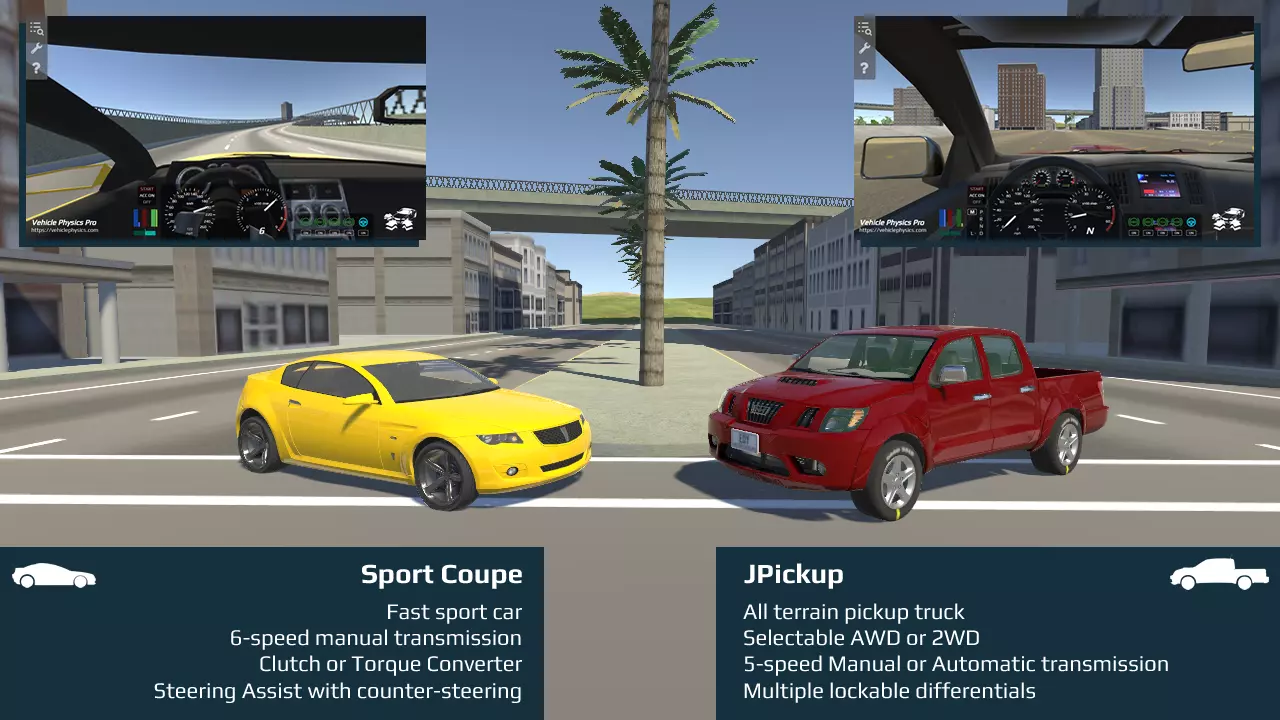
\includegraphics[width=14cm]{resources/figures/vpp-car-models.png}
\caption{Modele samochodów dostarczane w pakiecie Vehicle Physics Pro}
\source{https://assetstore.unity.com/packages/tools/physics/vehicle-physics-pro-community-edition-153556}
\label{VppCarModels}
\end{center}
\end{figure}

\newpage
\subsection{Tory wyścigowe}
\label{RaceTracksSection}
Na potrzeby implementacji systemu wybrałem dwa tory z pakietu \textbf{Environmental Race Track Pack}: ,,\textit{Figure 8 Track}'' oraz ,,\textit{Coastal Race Track}''. Tory uległy delikatnym modyfikacjom, polegającym przede wszystkim na usunięciu niepotrzebnych elementów sceny oraz zmianie jej oświetlenia. Widok torów z lotu ptaka został uwieczniony na rysunku \ref{RaceTracksFig}. \\

\begin{figure}[h]
\begin{center}
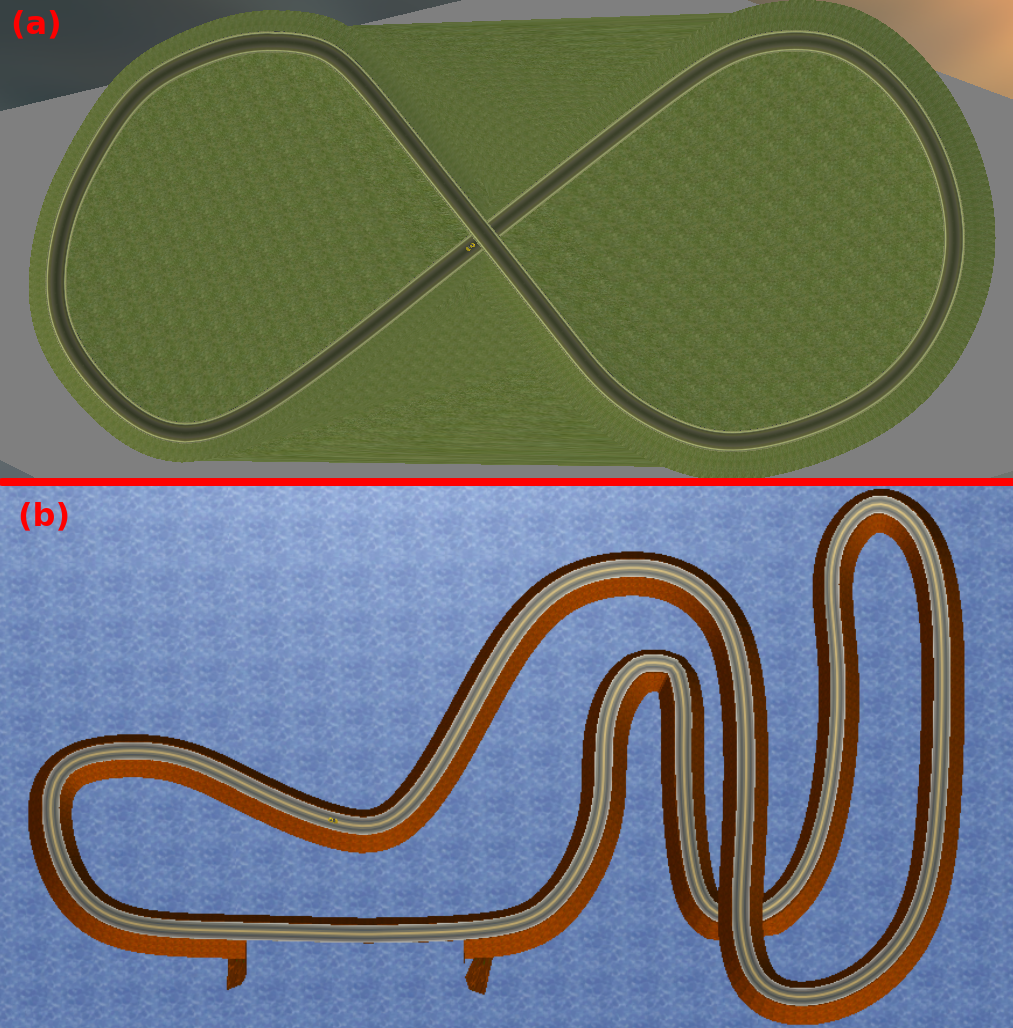
\includegraphics[width=14.5cm]{resources/figures/race_tracks_marked.png}
\caption{Tory wyścigowe wykorzystane w projekcie.}
\vspace*{-0.3cm}
\caption*{(a) Tor nr 1 - zmodyfikowany ,,\textit{Figure 8 Track}''}
\vspace*{-0.3cm}
\caption*{(b) Tor nr 2 - zmodyfikowany ,,\textit{Coastal Race Track}''}
\label{RaceTracksFig}
\end{center}
\end{figure}

\vspace{-0.5cm}
Tory różnią się od siebie przede wszystkim poziomem trudności - tor nr 2 wymaga od kierowcy znacznie większych umiejętności, ponieważ zakręty są bardziej zróżnicowane.

\subsection{Konfiguracja sceny Unity}
Na potrzeby eksperymentów obliczeniowych przygotowano kilka scen Unity. Zasadniczo różnią się one detalami, które dokładniej zostaną przedstawione w rozdziale \ref{ExperimentsChapter}-tym, natomiast ich rdzeń jest wszędzie taki sam. Najważniejszym obiektem na scenie jest \texttt{CarAgent}, reprezentujący model samochodu sterowany przez sieć neuronową. Obiekt składa się z kiku komponentów, wśród których najważniejsze to:
\vspace{-0.5cm}
\begin{enumerate*}
\item \textbf{Vehicle Controller} - komponent importowany z zestawu Vehicle Physics Pro (por. \ref{VppSection}). Odpowiada za ustawienia fizyki kluczowych elementów samochodu, takich jak: układ kierowniczy, hamulce, opony i skrzynia biegów \cite{vpp:vehicleController}. Na potrzeby implementacji systemu wprowadziłem następujące zmiany w konfiguracji komponentu:
\begin{itemize*}
\item Zmiana skrzyni biegów na automatyczną oraz wyzerowanie wartości parametrów ,,\textit{Gear transition time}'' oraz ,,\textit{Shift interval}'';
\item Wyłączenie wspomagania kierownicy i systemów wspomagania jazdy: kontroli trakcji (TCS), kontroli stabilności (ESC) oraz zapobiegania nadmiernemu uślizgowi kół (ASR).
\end{itemize*}
\item \textbf{Behavior Parameters} - komponent importowany z zestawu Unity ML-Agents (por. \ref{UnityMlSection}). Jego celem jest określenie wartości dla kluczowych parametrów trenowanego zachowania, takich jak rozmiar wektora obserwacji oraz rozmiar wektora akcji. Wartości te ulegały zmianie dla poszczególnych eksperymentów obliczeniowych, dlatego ten aspekt implementacji zostanie dokładniej opisany w kolejnym rozdziale.
\item \textbf{Klasa dziedzicząca po klasie Agent} - skrypt C\#, w którym zawarto implementację klasy dziedziczącej po klasie \texttt{Agent}, wywodzącej się z zestawu Unity ML-Agents. Na potrzeby eksperymentów obliczeniowych przygotowano kilka wersji implementacji tego skryptu, jednak rdzeń odpowiedzialności pozostaje taki sam. Skrypt jest odpowiedzialny za: prawidłową inicjalizację każdego epizodu treningu, przekazywanie obserwacji ze Środowiska Uczenia do sieci neuronowej, przekazywanie wyjścia z sieci neuronowej do Środowiska Uczenia oraz obliczanie wartości sygnałów nagrody dla danego kroku symulacji. Oprócz tego, każda wersja implementacji posiada własne, dodatkowe odpowiedzialności.
\item \textbf{Decision Requester} - komponent importowany z zestawu Unity ML-Agents. Jego głównym zadaniem jest określenie częstotliwości podejmowania decyzji przez Agenta.
\item \textbf{Camera Sensor} - czujnik kamery, importowany z zestawu Unity ML-Agents. Jest niezbędny, jeśli chcemy dostarczać sieci neuronowej obserwacje wizualne ze środowiska. Parametrami komponentu są m.in. wymiary obrazu oraz typ kompresji.
\end{enumerate*}

\section{Narzędzie mlagents\_learn}
Główne narzędzie do treningu sieci neuronowych, oferowane przez zestaw Unity ML-Agents \cite{unitymla:trainingMlAgents}. Parametry są przekazywane do narzędzia poprzez wiersz poleceń oraz plik konfiguracyjny utrzymany w formacie YAML \cite{unitymla:configFile}. Zestaw ustawień oraz hiperparametrów zdefiniowanych w pliku konfiguracyjnym zależy w ogromnym stopniu od zastosowanej metody treningowej oraz sposobu konfiguracji Środowiska Uczenia. Konkretna zawartość wykorzystanych plików konfiguracyjnych oraz użyte parametry wywołania narzędzia zostaną zaprezentowane w kolejnym rozdziale.

Wywołanie narzędzia skutkuje uruchomieniem procesu treningowego oraz rozpoczęciem uczenia sieci. W wyniku swojej pracy, proces treningowy generuje trzy artefakty:
\begin{enumerate*}
\item \textbf{Podsumowania} - metryki treningowe, aktualizowane podczas trwania treningu. Są bardzo pomocne przy monitorowaniu wyników uczenia sieci oraz ewentualnych aktualizacjach wartości hiperparametrów. Podsumowania można wyświetlić w eleganckiej formie graficznej, wykorzystując w tym celu narzędzie \textit{TensorBoard} \cite{unitymla:tensorboard}.
\item \textbf{Modele} - katalog z punktami kontrolnymi modelu aktualizowanego podczas szkolenia, a także ostateczny plik modelu. Plik ostateczny jest generowany jednorazowo, czyli po zakończeniu lub przerwaniu uczenia. Wszystkie wygenerowane modele są plikami w formacie ONNX \cite{onnx:website}.
\item \textbf{Pliki timerów} - zawierają zagregowane metryki procesu uczenia, w tym czas spędzony na określonych blokach kodu. Są bardzo pomocne podczas prac nad poprawą wydajności obliczeń procesu uczenia.
\end{enumerate*}

\subsection*{Trening sieci}
Podczas wszystkich eksperymentów obliczeniowych wykorzystywałem do treningu sieci metodę uczenia maszynowego o nazwie \textbf{uczenie ze wzmocnieniem} (z ang. \textit{reinforcement learning}). Zestaw narzędziowy Unity ML-Agents dostarcza implementacji dla dwóch algorytmów wspierających tę metodę - PPO \cite{ppo:opis} oraz SAC \cite{sac:opis}. Po kilku próbach okazało się, że dla moich potrzeb znacznie lepiej sprawdza się algorytm PPO, dlatego właśnie on został przeze mnie użyty we wszystkich eksperymentach obliczeniowych opisanych w rozdziale \ref{ExperimentsChapter}-tym. PPO jest wyjątkowe pośród innych algorytmów uczenia ze wzmocnieniem, ponieważ zachowuje balans pomiędzy łatwością implementacji, złożonością próbki oraz łatwością dostrajania. Z tego też powodu jest oferowany jako domyślny algorytm uczenia ze wzmocnieniem dla zestawu Unity ML-Agents.
\chapter{Eksperymenty obliczeniowe}
\label{ExperimentsChapter}
\vspace*{-1cm}
W tym rozdziale zostanie zaprezentowana część praktyczna tworzonej pracy, która polega na przeprowadzeniu kilku eksperymentów obliczeniowych w oparciu o przygotowane przez autora oprogramowanie. Rozdział rozpoczyna się od omówienia przyjętej metodyki eksperymentów, następnie zostaną przedstawione najistotniejsze szczegóły implementacyjne poszczególnych eksperymentów obliczeniowych. Rozdział zakończy się analizą uzyskanych wyników oraz opisem wypływających z tego wniosków.

\section{Metodyka eksperymentów}
W ramach opracowania metodyki eksperymentów obliczeniowych, autor pracy przyjął następujące założenia:
\begin{enumerate*}
\item Każdy eksperyment obliczeniowy polega na wytrenowaniu konwolucyjnej sieci neuronowej w przygotowanym Środowisku Uczenia. Po skończonym treningu, model podlega ewaluacji poprzez ocenę jego zachowania podczas jazdy po torze wyścigowym.
\item Konfiguracja treningu sieci neuronowej musi być zdefiniowana w pliku tekstowym o formacie akceptowanym przez narzędzie \texttt{mlagents\_learn}. Ścieżka do pliku będzie określana przy starcie treningu, jako jeden z parametrów wywołania narzędzia \texttt{mlagents\_learn}.
\item Wynikiem przeprowadzonego treningu sieci konwolucyjnej powinien być plik z wytrenowanym modelem.
\item Do samodzielnego przeprowadzenia eksperymentów obliczeniowych należy mieć zainstalowane odpowiednie narzędzia (zgodnie z opisem z rozdziału \ref{DesignSystemChapter}-ciego), jak również posiadać kod źródłowy aplikacji wymaganej do wykonania eksperymentów.
\item Wytrenowany model sieci neuronowej powinien posiadać format danych pozwalający na jego wizualizację przy użyciu zewnętrznego oprogramowania.
\end{enumerate*}

\section{Opis implementacji}
Implementacja systemu została częściowo opisana w rozdziale \ref{ImplementationChapter}-tym, natomiast każdy z przeprowadzonych eksperymentów wymagał dostosowania pewnych detali w implementacji. Poniżej zamieszczam opis tych elementów implementacji, które nie zostały jeszcze opisane, a są zbyt ważne aby je pominąć.

\subsection{Środowiska Uczenia}
\label{LearningEnvsSubsection}
W ramach prac nad częścią eksperymentalną zostały przygotowane 3 Środowiska Uczenia, będące niczym innym jak scenami silnika Unity. Każde Środowisko Uczenia posiada własną charakterystykę oraz pewne cechy szczególne, wyróżniające je na tle pozostałych Środowisk.

\subsubsection{RaceTrack\_1}
Te Środowisko Uczenia zostało oparte na torze wyścigowym ,,\textit{Figure 8 Track}'' z pakietu \textbf{Environmental Race Track Pack} (por. \ref{RaceTracksSection}). Najważniejszą cechą Środowiska jest brak oświetlenia, co zostało dołożone w kolejnych Środowiskach. Wykorzystaną tutaj implementacją klasy Agent jest \textit{SimpleCarAgent} (por. \ref{AgentImplementations}). Rysunek \ref{RaceTrack1AgentComps} przedstawia najważniejsze komponenty obiektu sceny \textit{CarAgent}. \\
\begin{figure}[h]
\begin{center}
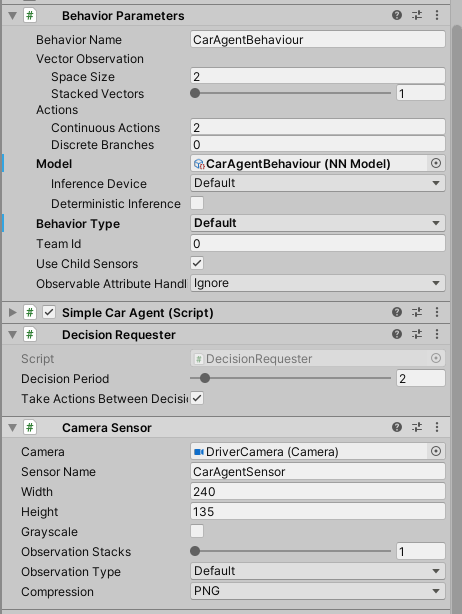
\includegraphics[width=9cm]{resources/figures/race_track_1_agent_components.png}
\caption{Najważniejsze komponenty obiektu \textit{CarAgent} w Środowisku Uczenia \textit{RaceTrack\_1}}
\label{RaceTrack1AgentComps}
\end{center}
\end{figure}
\noindent
Na podstawie rysunku można wysnuć kilka wniosków:
\vspace{-0.5cm}
\begin{itemize*}
\item Do agenta są dostarczane dwie obserwacje wektorowe;
\item Agent jest zobligowany do wykonywania dwóch akcji dla każdego kroku symulacji;
\item Wykorzystaną implementacją klasy \textit{Agent} jest klasa \textit{SimpleCarAgent};
\item Decyzje są podejmowane dla co drugiego kroku symulacji. Pomiędzy decyzjami należy wykonywać ostatnio obliczone Akcje;
\item Wykorzystywane są obserwacje wizualne w postaci pojedynczego czujnika, zbierającego obraz z kamery umieszczonej na miejscu fotela kierowcy. Obserwacje wizualne mają rozdzielczość $240 \times 135$ pikseli. Rysunek \ref{RaceTrack1Cockpit} przedstawia widok z kamery stanowiącej źródło danych wejściowych dla obserwacji wizualnych.
\end{itemize*}

\begin{figure}[h]
\begin{center}
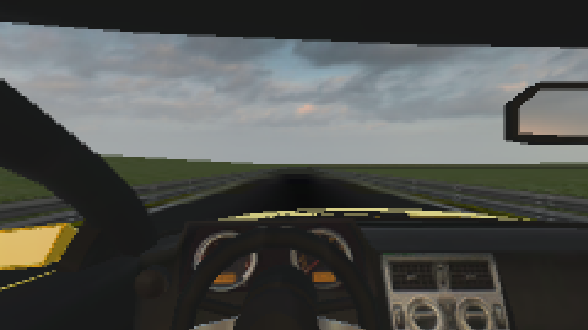
\includegraphics[width=15cm]{resources/figures/race_track_1_cockpit.png}
\caption{Widok z fotela kierowcy w Środowisku Uczenia \textit{RaceTrack\_1}}
\label{RaceTrack1Cockpit}
\end{center}
\vspace*{-1cm}
\end{figure}

\subsubsection{RaceTrack\_2}
Jest to Środowisko \textit{RaceTrack\_1} z dodanym oświetleniem kierunkowym, którego parametry są losowo ustawiane przed rozpoczęciem każdego epizodu symulacji. Parametry oświetlenia ulegające zmianie to \textbf{pozycja}, \textbf{rotacja} (orientacja), \textbf{kolor} oraz \textbf{intensywność}.

\subsubsection{RaceTrack\_3}
Środowisko Uczenia oparte na torze wyścigowym ,,,\textit{Coastal Race Track}'' z pakietu \textbf{Environmental Race Track Pack} (por. \ref{RaceTracksSection}). Ponieważ tor wyścigowy jest bardziej skomplikowany, przygotowana została nowa implementacja klasy \textit{Agent} - klasa \textit{AdvancedCarAgent}. Reszta komponentów obiektu sceny \textit{CarAgent} pozostała bez zmian. Rysunek \ref{RaceTrack3Cockpit} przedstawia widok z kamery dla tego Środowiska Uczenia. \\

\begin{figure}[h]
\begin{center}
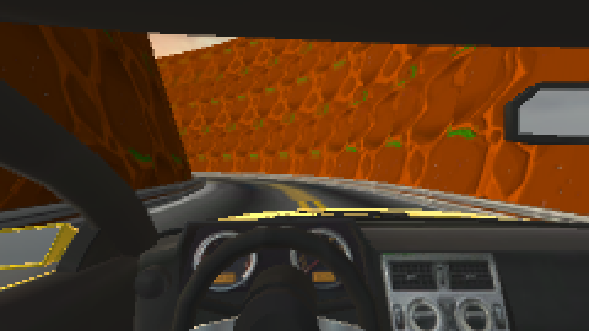
\includegraphics[width=15cm]{resources/figures/race_track_3_cockpit.png}
\caption{Widok z fotela kierowcy w Środowisku Uczenia \textit{RaceTrack\_3}}
\label{RaceTrack3Cockpit}
\end{center}
\end{figure}

\subsection{Implementacje klasy Agent}
\label{AgentImplementations}
W toku prac nad aplikacją zostało napisanych i przetestowanych wiele wersji implementacji klasy \textit{Agent} z zestawu Unity ML-Agents, jednak ostatecznie do wykorzystania zostały wyznaczone dwie klasy: \textit{SimpleCarAgent} oraz \textit{AdvancedCarAgent}. Chociaż są do siebie podobne, to jednak istnieje kilka różnic na które koniecznie trzeba zwrócić uwagę.

\subsubsection{SimpleCarAgent}
Klasa użyta w Środowiskach Uczenia \textit{RaceTrack\_1} oraz \textit{RaceTrack\_2} (por. \ref{LearningEnvsSubsection}). Jest odpowiedzialna za:
\begin{enumerate*}
\item \textit{Prawidłową inicjalizację każdego epizodu treningu} - przywrócenie samochodu do pozycji startowej oraz zmianę właściwości oświetlenia (jego pozycji, orientacji, koloru oraz intensywności).
\item \textit{Przekazywanie obserwacji ze Środowiska Uczenia do sieci neuronowej} - pobierane są 3 obserwacje ze środowiska - jedna wizualna (obraz z kamery) oraz dwie wektorowe (znormalizowana prędkość samochodu oraz informacja o tym, czy w danej chwili samochód dotyka jakiejś przeszkody).
\item \textit{Przekazywanie wyjścia z sieci neuronowej do Środowiska Uczenia} - sieć neuronowa generuje dwie wartości (zwane Akcjami), które są liczbami rzeczywistymi z domkniętego przedziału od $-1$ do $1$. Pierwsza wartość to stopień wciśnięcia pedału hamulca lub przepustnicy (gdzie $-1$ to maksymalnie wciśnięty hamulec, a $1$ to maksymalnie wciśnięta przepustnica), a druga to kąt skrętu kierownicy (gdzie $0$ oznacza jazdę na wprost, $-1$ maksymalny skręt w lewo a $1$ maksymalny skręt w prawo).
\item \textit{Obliczanie wartości sygnałów nagrody dla danego kroku symulacji} - sygnały nagród są obliczane na podstawie dwóch przesłanek: prędkości samochodu oraz kolizji z przeszkodami. Nagroda za prędkość jest proporcjonalna do prędkości samochodu, co oznacza że większa prędkość oznacza większą nagrodę. Za kolizje z przeszkodami przyznawane są kary, proporcjonalne do prędkości z jaką doszło do kolizji z przeszkodą. Dodatkowo przyznawana jest kara o stałej wartości za każdy krok symulacji, w którym samochód styka się z jakąś przeszkodą.
\end{enumerate*}
\noindent
Zmienne publiczne, jakie można przypisać do tej klasy z poziomu edytora Unity, to:
\vspace*{-0.5cm}
\begin{itemize*}
\item \texttt{MaxStep} - maksymalna liczba kroków symulacji dla danego epizodu;
\item \texttt{CarAgentObject} - Referencja na obiekt sceny \textit{CarAgent};
\item \texttt{StartCarPosition} - Pozycja początkowa samochodu;
\item \texttt{StartCarRotation} - Orientacja początkowa samochodu;
\item \texttt{DirectionalLight} - Referencja na obiekt oświetlenia (może być pusta, jeśli oświetlenie nie jest używane).
\end{itemize*}

\subsubsection{AdvancedCarAgent}
Klasa użyta w Środowisku Uczenia \textit{RaceTrack\_3} (por. \ref{LearningEnvsSubsection}). Posiada dokładnie te same odpowiedzialności co klasa \textit{SimpleCarAgent}, jak również większość kodu jest taka sama. Główna różnica polega na tym, że klasa \textit{AdvancedCarAgent} wspiera możliwość resetowania samochodu przy starcie nowego epizodu do wielu różnych pozycji oraz orientacji. Listę pozycji i orientacji można uzupełniać z poziomu edytora Unity, co widać na rysunku \ref{AdvancedCarAgentLocList}, gdzie został zaprezentowany fragment listy \texttt{StartCarLocations}. \\

\begin{figure}[h]
\begin{center}
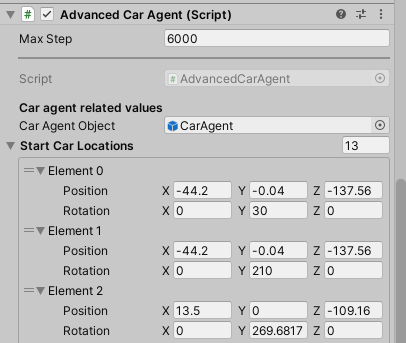
\includegraphics[width=6.5cm]{resources/figures/advanced_car_agent_loc_list.png}
\caption{\textit{AdvancedCarAgent} - fragment listy \texttt{StartCarLocations}.}
\label{AdvancedCarAgentLocList}
\end{center}
\end{figure}

\subsection{Konfiguracja treningu}
Konfiguracja treningu odbywa się poprzez przygotowanie pliku konfiguracyjnego w formacie YAML \cite{unitymla:configFile}. Dla każdego Środowiska Uczenia został przygotowany osobny plik konfiguracyjny, jednak różnice pomiędzy nimi są kosmetyczne i dotyczą detali. Oto zawartość pliku konfiguracyjnego dla Środowiska \textit{RaceTrack\_3}:

\begin{minted}[ fontsize=\fontsize{10}{9} ] {yaml}
engine_settings:
  width: 240
  height: 135
  quality_level: 5
  time_scale: 20
  target_frame_rate: -1
  capture_frame_rate: 60
  no_graphics: false
torch_settings:
  device: cuda
behaviors:
  CarAgentBehaviour:
    trainer_type: ppo
    summary_freq: 50000
    time_horizon: 256
    max_steps: 30000000
    keep_checkpoints: 10
    checkpoint_interval: 500000
    threaded: true
    network_settings:
      hidden_units: 128
      num_layers: 2
      normalize: true
      vis_encode_type: simple
      conditioning_type: none
    reward_signals:
      extrinsic:
        strength: 1.0
        gamma: 0.99
\end{minted}

Najważniejsze ustawienia dotyczą sekcji \texttt{behaviors}, ponieważ one mają największy wpływ na kształt treningu. W tym miejscu warto omówić kilka z nich:
\begin{enumerate*}
\item \texttt{trainer\_type} - wybór algorytmu uczącego. Dla wszystkich eksperymentów obliczeniowych wybrano algorytm PPO \cite{ppo:opis}, ponieważ w toku prac nad aplikacją okazał się być lepszym wyborem niż SAC \cite{sac:opis};
\item \texttt{time\_horizon} - jak wiele kroków symulacji należy zebrać przed dodaniem ich do ,,bufora doświadczenia''. Wartość parametru powinna znajdować się w kompromisie pomiędzy mniej stronniczym, ale wyższym oszacowaniem wariancji (długi horyzont czasowy) i bardziej stronniczym, ale mniej zróżnicowanym oszacowaniem (krótki horyzont czasowy). Gdy nagrody są często przyznawane lub epizody trwają dość długo, wtedy mniejsza liczba może być lepszym wyborem. Niemniej jednak, wartość ta powinna być na tyle duża, aby można było uchwycić wszystkie ważne zachowania w sekwencji działań agenta;
\item \texttt{max\_steps} - maksymalna liczba kroków symulacji przed zakończeniem treningu;
\item \texttt{keep\_checkpoints} - maksymalna liczba modeli sieci neuronowych, pozostawionych do zapisu. Modele te są zapisywane w odstępach określonych wartością parametru \texttt{checkpoint\_interval}, która oznacza interwał czasowy wyrażony w krokach symulacji treningowej; 
\item \texttt{network\_settings} - ustawienia sieci neuronowej. Najważniejsze z nich to:
\begin{itemize*}
\item \texttt{hidden\_units} - liczba neuronów w pełni połączonej warstwie ukrytej;
\item \texttt{num\_layers} - liczba warstw ukrytych;
\item \texttt{vis\_encode\_type} - typ enkodera dla obserwacji wizualnych.
\end{itemize*}
\end{enumerate*}

Rozpoczęcie treningu sieci odbywa się poprzez wywołanie komendy \texttt{mlagents\_learn}, której dokładne wykorzystanie zostało opisane w dokumentacji zestawu Unity ML-Agents \cite{unitymla:trainingMlAgents}.

\section{Przebieg eksperymentów i analiza wyników}
Dla każdego z przygotowanych Środowisk Uczenia przeprowadzono dokładnie jeden eksperyment obliczeniowy, polegający na wytrenowaniu konwolucyjnej sieci neuronowej do jazdy samochodem po wybranym torze wyścigowym, a następnie ewaluacji wytrenowanego modelu pod kątem przystosowania do rzeczywistej funkcji celu, jaką jest pokonanie toru wyścigowego w możliwie najkrótszym czasie.

\subsection{RaceTrack\_1}
Środowisko najłatwiejsze do wytrenowania konwolucyjnej sieci neuronowej, ponieważ brak jest zmiennego oświetlenia sceny, a zakręty są łagodne i niewymagające trudnych manewrów do wykonania. Wytrenowanie modelu zajęło 1 647 798 kroków symulacji. \\
Obserwacje sieci obejmowały:
\begin{enumerate*}
\item Obserwacje wizualne z kamery umieszczonej na fotelu kierowcy, czyli obrazki RGB o wymiarach $240 \times 135$ pikseli;
\item Obserwacje wektorowe:
\begin{itemize*}
\item Bieżąca, znormalizowana prędkość samochodu;
\item Wartość logiczna informująca, czy samochód w danej chwili styka się z jakąś przeszkodą.
\end{itemize*}
\end{enumerate*}

Model był trenowany na pojedynczej instancji obiektu sceny \textit{CarAgent}, którego pozycja i orientacja były resetowane na początku każdego epizodu symulacji. Epizod kończył się w momencie przejechania pełnego okrążenia lub po wyczerpaniu zakładanego limitu czasowego dla danego epizodu. Z testów wytrenowanego modelu wynika, że:
\begin{enumerate*}
\item Model charakteryzuje się niestabilnym tempem jazdy, a wykonane pomiary czasowe wskazują na dość znaczne odchyły w czasach okrążeń.
\item Wytrenowany model jest w stanie bezpiecznie przejechać kilka okrążeń pod rząd, choć ma tendencje do bardzo agresywnego wchodzenia w pierwszy zakręt, co czasem kończy się poważną kraksą - samochód obraca się o 90 stopni w stosunku do zakładanego kierunku jazdy.
\item Po wystąpieniu poważnej kraksy, wytrenowany model nie potrafi zazwyczaj wrócić do dalszej jazdy, lecz stara się zminimalizować straty poprzez oddalenie się od barierki, tak aby nie było naliczanej kary za kontakt z przeszkodami.
\item Model radzi sobie z jazdą tylko wtedy, gdy kolor drogi wyraźnie kontrastuje z poboczem - przy załączonym oświetleniu kierunkowym sieć się gubi, dojeżdżając do miejsca gdzie droga zbyt się rozjaśnia z powodu oświetlenia.
\end{enumerate*}

\subsection{RaceTrack\_2}
Środowisko Uczenia bardzo podobnie skonfigurowane do \textit{RaceTrack\_1}, jednak z jedną zasadniczą różnicą - trening odbywał się przy załączonym oświetleniu kierunkowym, którego właściwości były losowo ustawiane dla każdego epizodu treningowego. Model został wytrenowany po 4 654 498 krokach symulacji. Obserwacje modelu wykazały, że:
\begin{enumerate*}
\item Jego tempo jazdy jest znacznie stabilniejsze od poprzedniego modelu, ponieważ różnice między najszybszym i najwolniejszym okrążeniem były średnio 4-krotnie mniejsze niż dla poprzedniego modelu.
\item Model wciąż wykazuje tendencje do agresywnego wchodzenia w pierwszy zakręt, co często kończy się poważną kraksą.
\item Po wystąpieniu poważnej kraksy (obrócenie o 90 stopni lub więcej), samochód staje w miejscu lub wręcz zawraca i zaczyna jechać ,,pod prąd''. Pod tym względem zachowanie tego modelu niezbyt odbiega od zachowania modelu poprzedniego.
\item Model dobrze sobie radzi ze zmiennym oświetleniem, chociaż wciąż się gubi dla niektórych przypadków brzegowych.
\end{enumerate*}

\subsection{RaceTrack\_3}
W tym Środowisku Uczenia trening potrwał znacznie dłużej niż na obydwu poprzednich Środowiskach razem wziętych i wyniósł 12 999 786 milionów kroków symulacji. Wynika to z faktu, że te Środowisko jest dużo trudniejsze do wytrenowania, ponieważ tor wyścigowy jest bardziej zróżnicowany i składa się z zakrętów o bardziej odmiennej charakterystyce. \\
Z obserwacji wytrenowanego modelu wynika, że:
\begin{enumerate*}
\item Jego zachowanie jest dosyć nierówne. Z jednej strony, zdarza się że przez dłuższy odcinek czasu samochód całkiem znośnie pokonuje kolejne zakręty, zwalniając przed ostrzejszymi nawrotami. Z drugiej strony, chwilę później na łagodniejszym zakręcie samochód potrafi uderzyć pełnym impetem w barierkę, obrócić się bokiem do drogi i dalej nie ruszyć.
\item Model wypracował sobie strategię utrzymania toru jazdy samochodu przy mocnym zderzeniu z barierką na ostrym zakręcie. W takich sytuacjach następuje skręt kierownicy do skrajnej pozycji w kierunku zakrętu - czyli przy zakręcie w lewo następuje maksymalny skręt kierownicą na lewo.
\item Jeśli samochód po zderzeniu z barierką nie został obrócony prostopadle do kierunku jazdy, lecz pod pewnym mniejszym kątem, to wtedy jest szansa że samochód powróci do dalszej jazdy. Jeśli jednak samochód obróci się o więcej niż 90 stopni, to nie zawróci, ponieważ model nie posiada żadnych informacji na temat tego, w którą stronę samochód powinien się poruszać. W najlepszym wypadku samochód ruszy w drugą stronę.
\item Podobnie jak poprzedni model, całkiem dobrze radzi sobie ze zmiennym oświetleniem.
\item Przejeżdżając przez ciasne nawroty, samochód zwalnia aby uniknąć kolizji. W skrajnych przypadkach potrafi całkowicie się zatrzymać i dalej nie ruszyć, pomimo tego że sytuacja pozwalałaby na dalszą jazdę.
\end{enumerate*}

\clearpage
\section{Analiza wytrenowanego modelu}
Model wytrenowany w Środowisku \textit{RaceTrack\_3} został załadowany do programu o nazwie Netron (por. \ref{NetronOpis}). Rysunek \ref{ModelVisualization} przedstawia wizualizację załadowanego modelu. \\

\begin{figure}[h]
\begin{center}
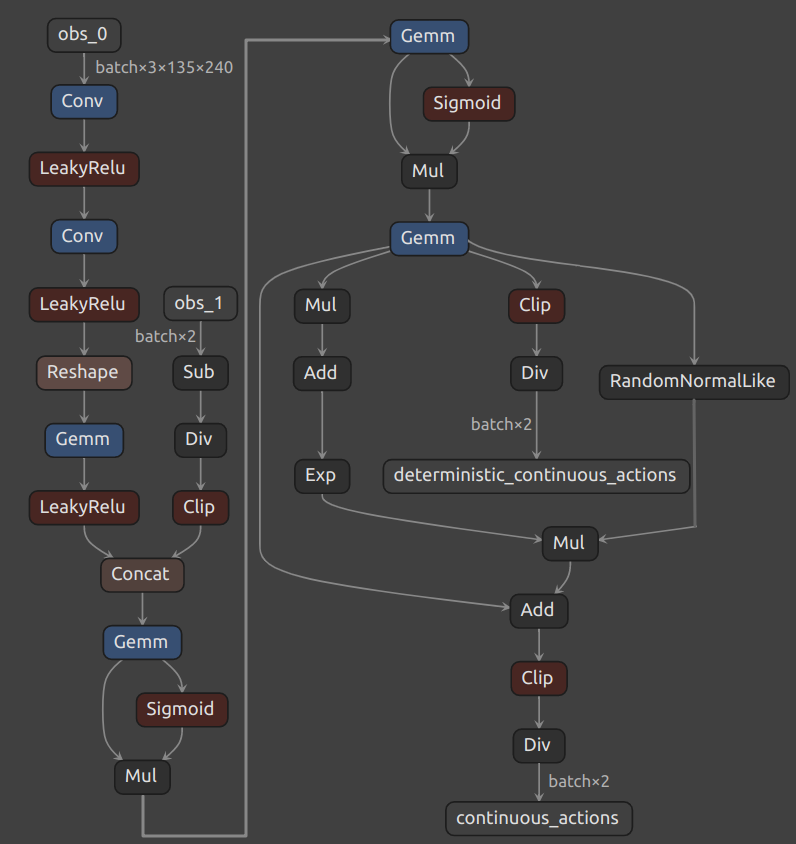
\includegraphics[width=13.5cm]{resources/figures/model_visualization.png}
\caption{Wizualizacja modelu wytrenowanego w Środowisku Uczenia \textit{RaceTrack\_3}}
\label{ModelVisualization}
\end{center}
\end{figure}

\begin{figure}[h]
\begin{center}
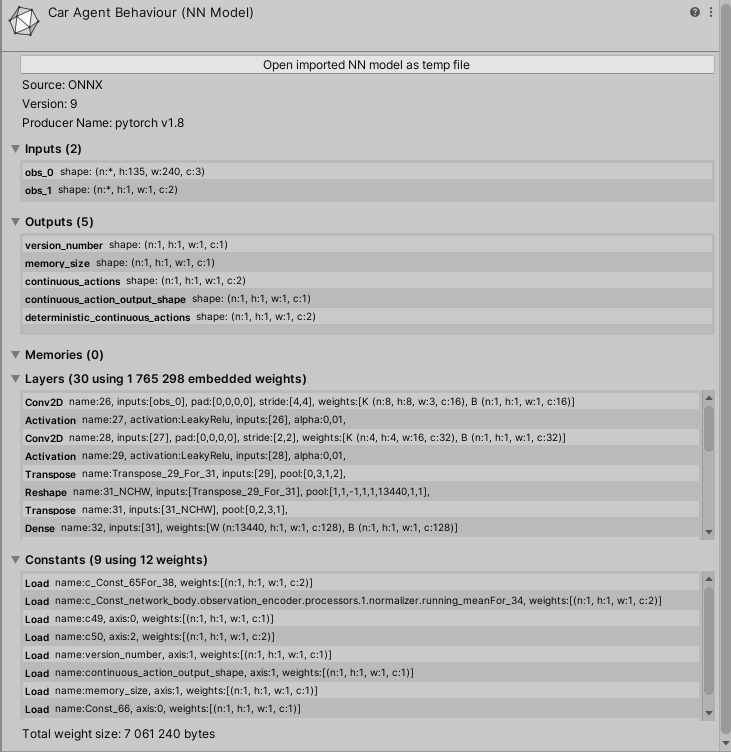
\includegraphics[width=13.5cm]{resources/figures/trained_model_inspector.png}
\caption{Podgląd wytrenowanego modelu w inspektorze edytora Unity}
\label{TrainedModelInspector}
\end{center}
\vspace*{-0.5cm}
\end{figure}

Więcej informacji na temat każdego z operatorów (czyli typów warstw sieci) można znaleźć na stronie dokumentacji standardu ONNX \cite{onnx:operators}. Wykorzystane operatory posiadają następujące znaczenie:
\vspace*{-0.5cm}
\begin{enumerate*}
\item \textbf{obs\_0}, \textbf{obs\_1} - obserwacje wejściowe (odpowiednio: wizualne i wektorowe);
\item \textbf{Conv} - warstwa konwolucyjna;
\item \textbf{LeakyRelu} - funkcja aktywacji LeakyRelu;
\item \textbf{Reshape} - warstwa zmieniająca kształt (wymiary) danych wejściowych;
\item \textbf{Add}, \textbf{Sub}, \textbf{Mul}, \textbf{Div} - operacje dodawania, odejmowania, mnożenia i dzielenia;
\item \textbf{Clip} - operacja obcinania wartości do zadanej dziedziny;
\item \textbf{Concat} - warstwa łącząca;
\item \textbf{Gemm} - warstwa ogólnego mnożenia macierzy;
\item \textbf{Sigmoid} - funkcja aktywacji Sigmoid;
\item \textbf{Exp} - operacja potęgowania;
\item \textbf{RandomNormalLike} - generator tensorów losowych.
\end{enumerate*}

Ten sam model można również podejrzeć w inspektorze edytora Unity, co zostało zaprezentowane na rysunku \ref{TrainedModelInspector}. Wytrenowany model składa się z 30 warstw oraz 1 765 298 wag, których wartości musiały zostać dostrojone podczas treningu. Cały plik modelu ma rozmiar 7 061 240 bajtów, co w przybliżeniu daje nam 6,73 MB.

W tym miejscu należy wyjaśnić, dlaczego zastosowano powyżej opisaną architekturę modelu sieci. Powody są następujące:
\begin{enumerate*}
\item Punktem wyjścia była chęć przeprowadzenia treningu w oparciu o dane wizualne, a do takich zadań doskonałym wyborem są konwolucyjne sieci neuronowe (por. rozdział \ref{CNNsChapter}-gi). Dlatego architektura sieci posiada warstwy konwolucyjne.
\item Dwie warstwy konwolucyjne są domyślnym wyborem, oferowanym przez zestaw Unity ML-Agents. Po  kilku testach, autor postanowił pozostać przy tej wartości, ponieważ okazała się być wystarczająco dobra dla potrzeb treningu.
\item Autor eksperymentował z różnymi rozdzielczościami obrazu wejściowego, rozpoczynając od możliwie najmniejszych wartości. Taki kierunek poszukiwań wydawał się właściwy, ponieważ mniejsze dane wejściowe oznaczają zwykle krótszy trening, a w konsekwencji szybszą ewaluację zaprojektowanego modelu. Jednakże zbyt niska rozdzielczość to brak detali istotnych do nauczenia się modelu, dlatego wybór właściwej rozdzielczości jest zawsze kwestią kompromisu. Po wielu testach, autor ostatecznie przyjął rozdzielczość $240 \times 135$, ponieważ przy niższej rozdzielczości ciasne nawroty były zauważane zbyt późno i model nie miał możliwości dohamować przed zakrętem.
\item Pozostałe elementy architektury sieci pochodzą z domyślnej konfiguracji zestawu Unity ML-Agent. Konfiguracja ta okazała się sprawdzać bardzo dobrze, dlatego autor pracy postanowił przy niej pozostać.
\end{enumerate*}

\section{Wnioski}
W wyniku przeprowadzonych eksperymentów obliczeniowych, autor niniejszej pracy sformułował kilka wniosków:

\begin{enumerate*}
\item Złożoność Środowiska Uczenia w bezpośredni sposób przekłada się na długość treningu sieci neuronowej. Pomimo braku zmian w topologii sieci, jej hiperparametrach czy też algorytmie uczącym, każde kolejne z opisanych Środowisk Uczenia wymagało zauważalnie więcej obliczeń podczas treningu modelu. Wynikało to z faktu, że każde kolejne Środowisko było bardziej różnorodne, co utrudniało algorytmowi uczącemu odnalezienie powiązań między wzorcami wizualnymi i oczekiwanymi akcjami.
\item Zaprojektowana funkcja nagród (zależna od prędkości samochodu oraz występujących kolizji) okazała się być wystarczająca jedynie dla wyuczenia się podstawowych manewrów, takich jak jazda po prostej oraz bezkolizyjne pokonywanie łagodnych zakrętów. Przejeżdżając przez ciaśniejsze zakręty, model wykazuje zbyt agresywne zachowanie, co zazwyczaj kończy się poważną stłuczką i brakiem możliwości dalszej jazdy. Aby to zmienić, funkcję nagród należałoby przeprojektować, co jest zadaniem wysoce nietrywialnym i wymagającym wiele czasu poświęconego na testowanie różnych rozwiązań.
\item Pomimo treningu przy zmiennym oświetleniu, rodzaj i natężenie oświetlenia wciąż mają istotny wpływ na jakość zachowania modelu.
\item Model wytrenowany na jednym Środowisku Uczenia nie potrafi się poprawnie zachować na pozostałych Środowiskach. Powodów takiego stanu rzeczy należałoby upatrywać w zauważalnych różnicach wizualnych pomiędzy Środowiskami.
\item Uzyskane wyniki eksperymentów pozwalają na zaobserwowanie korelacji pomiędzy Środowiskiem Uczenia a długością treningu, natomiast nie wnoszą żadnej wiedzy na temat wpływu konfiguracji na skuteczność wyuczonego modelu. Dalsze badania w tym zakresie są jak najbardziej wskazane.
\end{enumerate*}
\chapter*{Podsumowanie}
\addcontentsline{toc}{chapter}{Podsumowanie}
Celem pracy było stworzenie prostego systemu uczącego konwolucyjne sieci neuronowe na bazie symulacji uruchamianych w zaprojektowanym środowisku. Zadaniem wytrenowanych modeli była jazda wirtualnym modelem samochodu po przygotowanym torze wyścigowym. Trening sieci neuronowych odbywał się przy użyciu algorytmu PPO, wykorzystującego technikę uczenia maszynowego o nazwie \textbf{Uczenie ze Wzmocnieniem} (z ang. \textit{Reinforcement Learning}).

Cel pracy został osiągnięty w całości. Stworzona aplikacja pozwala na wytrenowanie sieci neuronowej na wybranym Środowisku Uczenia. Sieć konwolucyjna została z sukcesem wykorzystana do przetwarzania obserwacji wizualnych, pochodzących z kamery zamontowanej na fotelu kierowcy. Wytrenowane sieci neuronowe potrafią pokonywać wirtualne tory wyścigowe - nawet te o dużym stopniu skomplikowania. Więcej informacji o wytrenowanych modelach należy szukać w rozdziale \ref{ExperimentsChapter}-tym.

\section*{Perspektywy dalszych badań w dziedzinie}
Czas i wysiłek włożony w napisanie niniejszej pracy pozwolił na zaledwie pobieżne omówienie podjętego tematu. Uczenie maszynowe oraz projektowanie samochodów autonomicznych to dwa bardzo obszerne zagadnienia, na które wielu wybitnych naukowców poświęciło długie lata badań.

Jednym z oczywistych kierunków dalszych badań byłoby zastosowanie zdobytej wiedzy do wytrenowania modelu sterującego samochodem poruszającym się w prawdziwym świecie. Dla ułatwienia badań, eksperymenty należałoby rozpocząć od pojazdu o mniejszych gabarytach, czyli wykonanego w pewnej skali. Kolejny pomysł to dodanie większej liczby kamer, zamontowanych dookoła samochodu. Takie rozwiązanie doprowadziłoby do zwiększenia pola widzenia i pewniejszego zachowania podczas precyzyjnych manewrów, np. w ciasnych nawrotach lub podczas parkowania.

\addcontentsline{toc}{chapter}{Spis rysunków}
\listoffigures

%   this is for BibTeX
\bibliographystyle{plplain}
\bibliography{literatura}

%adds the bibliography to the table of contents
\addcontentsline{toc}{chapter}
         {\protect\numberline{Bibliografia\hspace{-96pt}}}
\end{document}